%**************************************%
%*    Generated from PreTeXt source   *%
%*    on 2019-07-27T23:20:10-06:00    *%
%*                                    *%
%*      https://pretextbook.org       *%
%*                                    *%
%**************************************%
\documentclass[twoside,11pt,]{book}
%% Custom Preamble Entries, early (use latex.preamble.early)
%% Default LaTeX packages
%%   1.  always employed (or nearly so) for some purpose, or
%%   2.  a stylewriter may assume their presence
\usepackage{geometry}
%% Some aspects of the preamble are conditional,
%% the LaTeX engine is one such determinant
\usepackage{ifthen}
%% etoolbox has a variety of modern conveniences
\usepackage{etoolbox}
\usepackage{ifxetex,ifluatex}
%% Raster graphics inclusion
\usepackage{graphicx}
%% Color support, xcolor package
%% Always loaded, for: add/delete text, author tools
%% Here, since tcolorbox loads tikz, and tikz loads xcolor
\PassOptionsToPackage{usenames,dvipsnames,svgnames,table}{xcolor}
\usepackage{xcolor}
%% Colored boxes, and much more, though mostly styling
%% skins library provides "enhanced" skin, employing tikzpicture
%% boxes may be configured as "breakable" or "unbreakable"
%% "raster" controls grids of boxes, aka side-by-side
\usepackage{tcolorbox}
\tcbuselibrary{skins}
\tcbuselibrary{breakable}
\tcbuselibrary{raster}
%% We load some "stock" tcolorbox styles that we use a lot
%% Placement here is provisional, there will be some color work also
%% First, black on white, no border, transparent, but no assumption about titles
\tcbset{ bwminimalstyle/.style={size=minimal, boxrule=-0.3pt, frame empty,
colback=white, colbacktitle=white, coltitle=black, opacityfill=0.0} }
%% Second, bold title, run-in to text/paragraph/heading
%% Space afterwards will be controlled by environment,
%% dependent of constructions of the tcb title
\tcbset{ runintitlestyle/.style={fonttitle=\normalfont\bfseries, attach title to upper} }
%% Spacing prior to each exercise, anywhere
\tcbset{ exercisespacingstyle/.style={before skip={1.5ex plus 0.5ex}} }
%% Spacing prior to each block
\tcbset{ blockspacingstyle/.style={before skip={2.0ex plus 0.5ex}} }
%% xparse allows the construction of more robust commands,
%% this is a necessity for isolating styling and behavior
%% The tcolorbox library of the same name loads the base library
\tcbuselibrary{xparse}
%% Hyperref should be here, but likes to be loaded late
%%
%% Inline math delimiters, \(, \), need to be robust
%% 2016-01-31:  latexrelease.sty  supersedes  fixltx2e.sty
%% If  latexrelease.sty  exists, bugfix is in kernel
%% If not, bugfix is in  fixltx2e.sty
%% See:  https://tug.org/TUGboat/tb36-3/tb114ltnews22.pdf
%% and read "Fewer fragile commands" in distribution's  latexchanges.pdf
\IfFileExists{latexrelease.sty}{}{\usepackage{fixltx2e}}
%% Text height identically 9 inches, text width varies on point size
%% See Bringhurst 2.1.1 on measure for recommendations
%% 75 characters per line (count spaces, punctuation) is target
%% which is the upper limit of Bringhurst's recommendations
\geometry{letterpaper,total={374pt,9.0in}}
%% Custom Page Layout Adjustments (use latex.geometry)
\geometry{papersize={7in,10in}, width=4.85in, inner=1in, height=8.5in, top=0.75in, twoside, ignoreheadfoot}
%% This LaTeX file may be compiled with pdflatex, xelatex, or lualatex executables
%% LuaTeX is not explicitly supported, but we do accept additions from knowledgeable users
%% The conditional below provides  pdflatex  specific configuration last
%% The following provides engine-specific capabilities
%% Generally, xelatex is necessary non-Western fonts
\ifthenelse{\boolean{xetex} \or \boolean{luatex}}{%
%% begin: xelatex and lualatex-specific configuration
\ifxetex\usepackage{xltxtra}\fi
%% realscripts is the only part of xltxtra relevant to lualatex 
\ifluatex\usepackage{realscripts}\fi
%% fontspec package provides extensive control of system fonts,
%% meaning *.otf (OpenType), and apparently *.ttf (TrueType)
%% that live *outside* your TeX/MF tree, and are controlled by your *system*
%% fontspec will make Latin Modern (lmodern) the default font
\usepackage{fontspec}
%% 
%% Extensive support for other languages
\usepackage{polyglossia}
%% Set main/default language based on pretext/@xml:lang value
%% document language code is "en-US", US English
%% usmax variant has extra hypenation
\setmainlanguage[variant=usmax]{english}
%% Enable secondary languages based on discovery of @xml:lang values
%% Enable fonts/scripts based on discovery of @xml:lang values
%% Western languages should be ably covered by Latin Modern Roman
%% end: xelatex and lualatex-specific configuration
}{%
%% begin: pdflatex-specific configuration
\usepackage[utf8]{inputenc}
%% PreTeXt will create a UTF-8 encoded file
%% begin: font setup and configuration for use with pdflatex
\usepackage{lmodern}
\usepackage[T1]{fontenc}
%% end: font setup and configuration for use with pdflatex
%% end: pdflatex-specific configuration
}
%% Monospace font: Inconsolata (zi4)
%% Sponsored by TUG: http://levien.com/type/myfonts/inconsolata.html
%% Loaded for documents with intentional objects requiring monospace
%% See package documentation for excellent instructions
%% One caveat, seem to need full file name to locate OTF files
%% Loads the "upquote" package as needed, so we don't have to
%% Upright quotes might come from the  textcomp  package, which we also use
%% We employ the shapely \ell to match Google Font version
%% pdflatex: "varqu" option produces best upright quotes
%% xelatex,lualatex: add StylisticSet 1 for shapely \ell
%% xelatex,lualatex: add StylisticSet 2 for plain zero
%% xelatex,lualatex: we add StylisticSet 3 for upright quotes
%% 
\ifthenelse{\boolean{xetex} \or \boolean{luatex}}{%
%% begin: xelatex and lualatex-specific monospace font
\usepackage{zi4}
\setmonofont[BoldFont=Inconsolatazi4-Bold.otf,StylisticSet={1,3}]{Inconsolatazi4-Regular.otf}
%% end: xelatex and lualatex-specific monospace font
}{%
%% begin: pdflatex-specific monospace font
%% "varqu" option provides textcomp \textquotedbl glyph
%% "varl"  option provides shapely "ell"
\usepackage[varqu,varl]{zi4}
%% end: pdflatex-specific monospace font
}
%% Symbols, align environment, bracket-matrix
\usepackage{amsmath}
\usepackage{amssymb}
%% allow page breaks within display mathematics anywhere
%% level 4 is maximally permissive
%% this is exactly the opposite of AMSmath package philosophy
%% there are per-display, and per-equation options to control this
%% split, aligned, gathered, and alignedat are not affected
\allowdisplaybreaks[4]
%% allow more columns to a matrix
%% can make this even bigger by overriding with  latex.preamble.late  processing option
\setcounter{MaxMatrixCols}{30}
%%
%%
%% Division Titles, and Page Headers/Footers
%% titlesec package, loading "titleps" package cooperatively
%% See code comments about the necessity and purpose of "explicit" option
\usepackage[explicit, pagestyles]{titlesec}
\newtitlemark{\chaptertitlename}
%% Set global/default page style for document due
%% to potential re-definitions after documentclass
\pagestyle{headings}
%%
%% Create globally-available macros to be provided for style writers
%% These are redefined for each occurence of each division
\newcommand{\divisionnameptx}{\relax}%
\newcommand{\titleptx}{\relax}%
\newcommand{\subtitleptx}{\relax}%
\newcommand{\shortitleptx}{\relax}%
\newcommand{\authorsptx}{\relax}%
\newcommand{\epigraphptx}{\relax}%
%% Create environments for possible occurences of each division
%% Environment for a PTX "chapter" at the level of a LaTeX "chapter"
\NewDocumentEnvironment{chapterptx}{mmmmmm}
{%
\renewcommand{\divisionnameptx}{Chapter}%
\renewcommand{\titleptx}{#1}%
\renewcommand{\subtitleptx}{#2}%
\renewcommand{\shortitleptx}{#3}%
\renewcommand{\authorsptx}{#4}%
\renewcommand{\epigraphptx}{#5}%
\chapter[#3]{#1}%
\label{#6}%
}{}%
%% Environment for a PTX "worksheet" at the level of a LaTeX "section"
\NewDocumentEnvironment{worksheet-section}{mmmmmm}
{%
\renewcommand{\divisionnameptx}{Worksheet}%
\renewcommand{\titleptx}{#1}%
\renewcommand{\subtitleptx}{#2}%
\renewcommand{\shortitleptx}{#3}%
\renewcommand{\authorsptx}{#4}%
\renewcommand{\epigraphptx}{#5}%
\section[#3]{#1}%
\label{#6}%
}{}%
%% Environment for a PTX "worksheet" at the level of a LaTeX "section"
\NewDocumentEnvironment{worksheet-section-numberless}{mmmmmm}
{%
\renewcommand{\divisionnameptx}{Worksheet}%
\renewcommand{\titleptx}{#1}%
\renewcommand{\subtitleptx}{#2}%
\renewcommand{\shortitleptx}{#3}%
\renewcommand{\authorsptx}{#4}%
\renewcommand{\epigraphptx}{#5}%
\section*{#1}%
\addcontentsline{toc}{section}{#3}
\label{#6}%
}{}%
%%
%% Styles for six traditional LaTeX divisions
\titleformat{\chapter}[display]
{\normalfont\huge\bfseries}{\divisionnameptx\space\thechapter}{20pt}{\Huge#1}
[{\Large\authorsptx}]
\titleformat{name=\chapter,numberless}[display]
{\normalfont\huge\bfseries}{}{0pt}{#1}
[{\Large\authorsptx}]
\titlespacing*{\chapter}{0pt}{50pt}{40pt}
\titleformat{\section}[hang]
{\normalfont\Large\bfseries}{\thesection}{1ex}{#1}
[{\large\authorsptx}]
\titleformat{name=\section,numberless}[block]
{\normalfont\Large\bfseries}{}{0pt}{#1}
[{\large\authorsptx}]
\titlespacing*{\section}{0pt}{3.5ex plus 1ex minus .2ex}{2.3ex plus .2ex}
\titleformat{\subsection}[hang]
{\normalfont\large\bfseries}{\thesubsection}{1ex}{#1}
[{\normalsize\authorsptx}]
\titleformat{name=\subsection,numberless}[block]
{\normalfont\large\bfseries}{}{0pt}{#1}
[{\normalsize\authorsptx}]
\titlespacing*{\subsection}{0pt}{3.25ex plus 1ex minus .2ex}{1.5ex plus .2ex}
\titleformat{\subsubsection}[hang]
{\normalfont\normalsize\bfseries}{\thesubsubsection}{1em}{#1}
[{\small\authorsptx}]
\titleformat{name=\subsubsection,numberless}[block]
{\normalfont\normalsize\bfseries}{}{0pt}{#1}
[{\normalsize\authorsptx}]
\titlespacing*{\subsubsection}{0pt}{3.25ex plus 1ex minus .2ex}{1.5ex plus .2ex}
\titleformat{\paragraph}[hang]
{\normalfont\normalsize\bfseries}{\theparagraph}{1em}{#1}
[{\small\authorsptx}]
\titleformat{name=\paragraph,numberless}[block]
{\normalfont\normalsize\bfseries}{}{0pt}{#1}
[{\normalsize\authorsptx}]
\titlespacing*{\paragraph}{0pt}{3.25ex plus 1ex minus .2ex}{1.5em}
%%
%% Semantic Macros
%% To preserve meaning in a LaTeX file
%%
%% \mono macro for content of "c", "cd", "tag", etc elements
%% Also used automatically in other constructions
%% Simply an alias for \texttt
%% Always defined, even if there is no need, or if a specific tt font is not loaded
\newcommand{\mono}[1]{\texttt{#1}}
%%
%% Following semantic macros are only defined here if their
%% use is required only in this specific document
%%
%% Division Numbering: Chapters, Sections, Subsections, etc
%% Division numbers may be turned off at some level ("depth")
%% A section *always* has depth 1, contrary to us counting from the document root
%% The latex default is 3.  If a larger number is present here, then
%% removing this command may make some cross-references ambiguous
%% The precursor variable $numbering-maxlevel is checked for consistency in the common XSL file
\setcounter{secnumdepth}{1}
%% begin: General AMS environment setup
%% Environments built with amsthm package
\usepackage{amsthm}
%% Numbering for Theorems, Conjectures, Examples, Figures, etc
%% Controlled by  numbering.theorems.level  processing parameter
%% Numbering: all theorem-like numbered consecutively
%% i.e. Corollary 4.3 follows Theorem 4.2
%% Always need some theorem environment to set base numbering scheme
%% even if document has no theorems (but has other environments)
%% Create a never-used style first, always
%% simply to provide a global counter to use, namely "cthm"
\newtheorem{cthm}{BadTheoremStringName}[section]
%% AMS "proof" environment is not used, but we leave previously
%% implemented \qedhere in place, should the LaTeX be recycled
\renewcommand{\qedhere}{\relax}
%% end: General AMS environment setup
%%
%% xparse environments for introductions and conclusions of divisions
%%
%% introduction: in a structured division
\NewDocumentEnvironment{introduction}{m}
{\notblank{#1}{\noindent\textbf{#1}\space}{}}{\par\medskip}
%% Divisional exercises (and worksheet) as LaTeX environments
%% Third argument is option for extra workspace in worksheets
%% Hanging indent occupies a 5ex width slot prior to left margin
%% Experimentally this seems just barely sufficient for a bold "888."
%% Division exercises, not in exercise group
\tcbset{ divisionexercisestyle/.style={bwminimalstyle, runintitlestyle, exercisespacingstyle, left=5ex, breakable, parbox=false } }
\newtcolorbox{divisionexercise}[4]{divisionexercisestyle, before title={\hspace{-5ex}\makebox[5ex][l]{#1.}}, title={\notblank{#2}{#2\space}{}}, phantom={\hypertarget{#4}{}}, after={\notblank{#3}{\newline\rule{\workspacestrutwidth}{#3\textheight}\newline}{}}}
%% Worksheet exercises may have workspaces
\newlength{\workspacestrutwidth}
%% @workspace strut is invisible
\setlength{\workspacestrutwidth}{0pt}
%% Localize LaTeX supplied names (possibly none)
\renewcommand*{\chaptername}{Chapter}
\setcounter{chapter}{-1}
%% "tcolorbox" environment for a single image, occupying entire \linewidth
%% arguments are left-margin, width, right-margin, as multiples of
%% \linewidth, and are guaranteed to be positive and sum to 1.0
\tcbset{ imagestyle/.style={bwminimalstyle} }
\NewTColorBox{image}{mmm}{imagestyle,left skip=#1\linewidth,width=#2\linewidth}
%% Figures, Tables, Listings, Named Lists, Floats
%% The [H]ere option of the float package fixes floats in-place,
%% in deference to web usage, where floats are totally irrelevant
%% You can remove some of this setup, to restore standard LaTeX behavior
%% HOWEVER, numbering of figures/tables AND theorems/examples/remarks, etc
%% may de-synchronize with the numbering in the HTML version
%% You can remove the "placement={H}" option to allow flotation and
%% preserve numbering, BUT the numbering may then appear "out-of-order"
%% Floating environments: http://tex.stackexchange.com/questions/95631/
\usepackage{float}
\usepackage{newfloat}
\usepackage{caption}%% Adjust stock figure environment so that it no longer floats
\SetupFloatingEnvironment{figure}{fileext=lof,placement={H},within=section,name=Figure}
\captionsetup[figure]{labelfont=bf,justification=raggedright}
%% http://tex.stackexchange.com/questions/16195
\makeatletter
\let\c@figure\c@cthm
\makeatother
%% More flexible list management, esp. for references
%% But also for specifying labels (i.e. custom order) on nested lists
\usepackage{enumitem}
%% hyperref driver does not need to be specified, it will be detected
%% Footnote marks in tcolorbox have broken linking under
%% hyperref, so it is necessary to turn off all linking
%% It *must* be given as a package option, not with \hypersetup
\usepackage[hyperfootnotes=false]{hyperref}
%% configure hyperref's  \url  to match listings' inline verbatim
\renewcommand\UrlFont{\small\ttfamily}
%% Hyperlinking active in electronic PDFs, all links solid and blue
\hypersetup{colorlinks=true,linkcolor=blue,citecolor=blue,filecolor=blue,urlcolor=blue}
\hypersetup{pdftitle={Mathematics for Elementary Teachers}}
%% If you manually remove hyperref, leave in this next command
\providecommand\phantomsection{}
%% Graphics Preamble Entries
\usepackage{tikz, pgfplots}
\usetikzlibrary{positioning,matrix,arrows}
\usetikzlibrary{shapes,decorations,shadows,fadings,patterns}
\usetikzlibrary{decorations.markings}
%% If tikz has been loaded, replace ampersand with \amp macro
%% tcolorbox styles for sidebyside layout
\tcbset{ sbsstyle/.style={raster equal height=rows,raster force size=false} }
\tcbset{ sbsheadingstyle/.style={bwminimalstyle, halign=center, fontupper=\bfseries} }
\tcbset{ sbspanelstyle/.style={bwminimalstyle} }
\tcbset{ sbscaptionstyle/.style={bwminimalstyle, halign=center} }
%% Enviroments for side-by-side and components
%% Necessary to use \NewTColorBox for boxes of the panels
%% "newfloat" environment to squash page-breaks within a single sidebyside
%% "xparse" environment for entire sidebyside
\NewDocumentEnvironment{sidebyside}{mmmm}
  {\begin{tcbraster}
    [sbsstyle,raster columns=#1,
    raster left skip=#2\linewidth,raster right skip=#3\linewidth,raster column skip=#4\linewidth]}
  {\end{tcbraster}}
%% "tcolorbox" environments for three components of a panel
\NewTColorBox{sbsheading}{m}{sbsheadingstyle,width=#1\linewidth}
\NewTColorBox{sbspanel}{mO{top}}{sbspanelstyle,width=#1\linewidth,valign=#2}
\NewTColorBox{sbscaption}{m}{sbscaptionstyle,width=#1\linewidth}
%% extpfeil package for certain extensible arrows,
%% as also provided by MathJax extension of the same name
%% NB: this package loads mtools, which loads calc, which redefines
%%     \setlength, so it can be removed if it seems to be in the 
%%     way and your math does not use:
%%     
%%     \xtwoheadrightarrow, \xtwoheadleftarrow, \xmapsto, \xlongequal, \xtofrom
%%     
%%     we have had to be extra careful with variable thickness
%%     lines in tables, and so also load this package late
\usepackage{extpfeil}
%% Custom Preamble Entries, late (use latex.preamble.late)
%% Begin: Author-provided packages
%% (From  docinfo/latex-preamble/package  elements)
%% End: Author-provided packages
%% Begin: Author-provided macros
%% (From  docinfo/macros  element)
%% Plus three from MBX for XML characters
\newcommand{\N}{\mathbb N}
\newcommand{\Z}{\mathbb Z}
\newcommand{\Q}{\mathbb Q}
\newcommand{\R}{\mathbb R}
\newcommand{\C}{\mathbb C}
\newcommand{\inv}{^{-1}}
\newcommand{\st}{:}
\renewcommand{\iff}{\leftrightarrow}
\newcommand{\Iff}{\Leftrightarrow}
\newcommand{\imp}{\rightarrow}
\newcommand{\Imp}{\Rightarrow}
\newcommand{\isom}{\cong}

\renewcommand{\bar}{\overline}
\newcommand{\card}[1]{\left| #1 \right|}
\newcommand{\lt}{<}
\newcommand{\gt}{>}
\newcommand{\amp}{&}
%% End: Author-provided macros
\begin{document}
\frontmatter
%% begin: half-title
\thispagestyle{empty}
{\centering
\vspace*{0.28\textheight}
{\Huge Mathematics for Elementary Teachers}\\[2\baselineskip]
{\LARGE A Workbook}\\
}
\clearpage
%% end:   half-title
%% begin: adcard
\thispagestyle{empty}
\null%
\clearpage
%% end:   adcard
%% begin: title page
%% Inspired by Peter Wilson's "titleDB" in "titlepages" CTAN package
\thispagestyle{empty}
{\centering
\vspace*{0.14\textheight}
%% Target for xref to top-level element is ToC
\addtocontents{toc}{\protect\hypertarget{x:book:workbook}{}}
{\Huge Mathematics for Elementary Teachers}\\[\baselineskip]
{\LARGE A Workbook}\\[3\baselineskip]
{\Large \textbraceleft{}author\textbraceright{}}\\[0.5\baselineskip]
{\Large \textbraceleft{}institution\textbraceright{}}\\[3\baselineskip]
{\Large July 27, 2019}\\}
\clearpage
%% end:   title page
%% begin: copyright-page
\thispagestyle{empty}
\hypertarget{g:colophon:idm35257947680}{}\vspace*{\stretch{2}}
\noindent{\bfseries Website}: \href{[website]}{\mono{[website]}}\par\medskip
\noindent\textcopyright{}[copyright-year]\quad{}[copyright-holder]\\[0.5\baselineskip]
 This work is licensed under the Creative Commons Attribution-ShareAlike 4.0 International License. To view a copy of this license, visit \href{http://creativecommons.org/licenses/by-sa/4.0/}{http:\slash{}\slash{}creativecommons.org\slash{}licenses\slash{}by-sa\slash{}4.0\slash{}}\par\medskip
\vspace*{\stretch{1}}
\null\clearpage
%% end:   copyright-page
%% begin: table of contents
%% Adjust Table of Contents
\setcounter{tocdepth}{2}
\renewcommand*\contentsname{Contents}
\tableofcontents
%% end:   table of contents
\mainmatter
%
%
\typeout{************************************************}
\typeout{Chapter 0 Worksheets}
\typeout{************************************************}
%
\begin{chapterptx}{Worksheets}{}{Worksheets}{}{}{g:chapter:idm35257985280}
%
%
\typeout{************************************************}
\typeout{Worksheet 0 A Trip to Quintopia!}
\typeout{************************************************}
%
\newgeometry{left=1.25cm, right=1.25cm, top=1.25cm, bottom=1.25cm}
\begin{worksheet-section-numberless}{A Trip to Quintopia!}{}{A Trip to Quintopia!}{}{}{x:worksheet:ws-quintopia-1-intro}
\begin{introduction}{}%
While on an Intergalactic Numismatics Tour, you encounter a meteor shower and are forced to make an unscheduled stop on the planet Quintopia.  The monetary system used in Quintopia consists of three coins:  a yellow coin (worth \textdollar{}1US), a red coin (worth five yellow coins), and a blue coin (worth five red coins).%
\par
Quintopia turns out to be a rather dull place to visit.  To help pass the time at the shuttle docking area, you and a fellow passenger play a game with the Quintopia currency.%
\end{introduction}%
\begin{divisionexercise}{1}{}{0.1}{g:exercise:idm35257929568}%
Coin Trading Game%
%
\begin{itemize}[label=\textbullet]
\item{}Materials:  Quintopia coins (yellow, red and blue), one die (number cube)%
\item{}Players:  2 or more%
\item{}Rules:%
\begin{itemize}[label=$\circ$]
\item{}The youngest player starts, and players alternate turns afterwards.%
\item{}On each turn, a player rolls the die and places that many yellow coins on his or her game sheet (see below).%
\item{}Whenever possible, a player MUST trade in five yellow coins for a red coin, or trade in five red coins for a blue coin, and place them in their respective columns.  As a result, no more than four coins of any one color should be a player’s game sheet.%
\item{}The first player to get two blue coins is the winner.%
\end{itemize}
%
\end{itemize}
\begin{sidebyside}{1}{0}{0}{0}%
\begin{sbspanel}{1}%
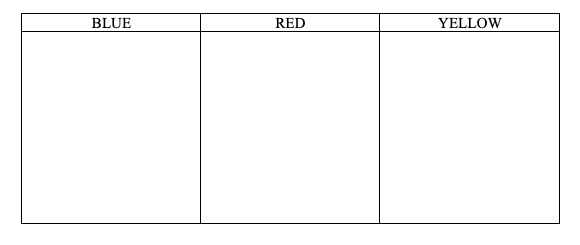
\includegraphics[width=1\linewidth]{images/quintopia-table.png}
\end{sbspanel}%
\end{sidebyside}%
\end{divisionexercise}%
\clearpage
\begin{divisionexercise}{2}{}{0.1}{g:exercise:idm35257921104}%
Coin Trading Game Revisited%
\par
A third passenger has been watching you play.  She suggests it is more challenging to start the game with TWO BLUE coins and to remove the number of yellow coins equal to the number rolled on each turn.  The first player to remove all of the coins from his or her playing board is the winner.  (Note: On the last turn, the number rolled may exceed the number of yellow chips remaining.)  Before you play this new version of the coin trading game, think about how you can remove yellow coins when you have none on your board (you only have two blue ones).  Note: Do not trade in coins until you absolutely need to.  For example, you should not immediately trade in your two blue coins all for red or yellow coins.%
\begin{sidebyside}{1}{0}{0}{0}%
\begin{sbspanel}{1}%
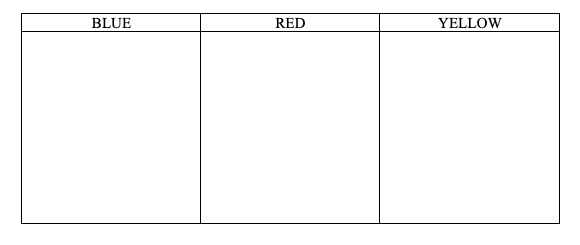
\includegraphics[width=1\linewidth]{images/quintopia-table.png}
\end{sbspanel}%
\end{sidebyside}%
%
\begin{description}
\item[{}]What do you notice?\item[{}]What do you wonder?\item[{}]What ideas and questions do you have?\end{description}
\end{divisionexercise}%
\end{worksheet-section-numberless}
\restoregeometry
%
%
\typeout{************************************************}
\typeout{Worksheet 0 Shopping in Quintopia}
\typeout{************************************************}
%
\newgeometry{left=1.25cm, right=1.25cm, top=1.25cm, bottom=1.25cm}
\begin{worksheet-section-numberless}{Shopping in Quintopia}{}{Shopping in Quintopia}{}{}{x:worksheet:ws-quintopia-2-shopping}
\begin{introduction}{}%
You got bored on the ship deck and decided to visit Quintopia to do some shopping. You know you can only use Quintopian currency while shopping, so you exchange some of your US dollars before your shopping and you have \(312_{5}\) (in Quintopian currency), which means 3 blue, 1 red, and 2 yellow coins. While you’re shopping, recall that whenever possible, you must trade in five yellow coins for a red coin, or trade in five red coins for a blue coin, and so on.%
\end{introduction}%
\begin{divisionexercise}{1}{}{0.15}{g:exercise:idm35257939152}%
Before you left the ship, you won a gift card worth \(24_{5}\) (in Quintopian currency). How much total money do you have now for shopping? Show your process in at least two different ways.%
\end{divisionexercise}%
\begin{divisionexercise}{2}{}{0.15}{g:exercise:idm35257913088}%
You spent \(43_{5}\) at the Appletopia store. How much Quintopian money do you have left?  Explain your process.%
\end{divisionexercise}%
\begin{divisionexercise}{3}{}{0.15}{g:exercise:idm35257911280}%
You saw a pair of shoes you like and it only costs \(32_{5}\). Since it is very cheap, you want to buy three pairs. How much will it cost to buy three pairs of shoes (in Quintopia currency)? Solve this question in two different ways.%
\end{divisionexercise}%
\clearpage
\begin{divisionexercise}{4}{}{0.15}{g:exercise:idm35257908896}%
After buying all three pairs of shoes, how much money do you have left?%
\end{divisionexercise}%
\begin{divisionexercise}{5}{}{0.15}{g:exercise:idm35257907344}%
After all your shopping you had some dinner which cost \(102_{5}\) . Do you have enough Quintopian money to pay? If not, how much Quintopian money do you need?  If you have an extra \textdollar{}6 US currency, will that be enough to pay the rest?%
\end{divisionexercise}%
\begin{divisionexercise}{6}{}{0.15}{g:exercise:idm35257905232}%
Discuss Base 5 and Base 10; and meaning of addition, subtraction and multiplication operations. Discuss expanded form.%
\end{divisionexercise}%
\end{worksheet-section-numberless}
\restoregeometry
%
%
\typeout{************************************************}
\typeout{Worksheet 0 Connections to Base Blocks}
\typeout{************************************************}
%
\newgeometry{left=1.25cm, right=1.25cm, top=1.25cm, bottom=1.25cm}
\begin{worksheet-section-numberless}{Connections to Base Blocks}{}{Connections to Base Blocks}{}{}{x:worksheet:ws-quintopia-3-base-connections}
\begin{divisionexercise}{1}{}{0.2}{g:exercise:idm35257940800}%
Using base-5 blocks, discuss how Quintopian currency would be represented. For example, represent \(314_{5}\) and \(43_{5}\). If you have \textdollar{}58 dollars how would you represent it using base-5 blocks?%
\end{divisionexercise}%
\begin{divisionexercise}{2}{}{0.2}{g:exercise:idm35257900592}%
If you have \(412_{5}\) in base-5 blocks and you trade in all the blocks for their corresponding number of small cubes, how many small cubes would you have?%
\end{divisionexercise}%
\begin{divisionexercise}{3}{}{0.15}{g:exercise:idm35257898784}%
Discuss with your group and note your conclusions.%
%
\begin{enumerate}[label=(\alph*)]
\item{}How do base-5 blocks compare to base-10?%
\item{}What are the place values worth in base-5 vs. base-10?%
\item{}What are the minimum and maximum number of blocks of each place value that you can have in base-5?%
\item{}What about base-10?%
\item{}How does this relate to the digits you can use to represent numbers in base-5 vs. base-10?%
\end{enumerate}
\end{divisionexercise}%
\begin{divisionexercise}{4}{}{0.1}{g:exercise:idm35257894144}%
Using base-10 blocks find the sum and the difference of 208 and 93.%
\end{divisionexercise}%
\begin{divisionexercise}{5}{}{0.1}{g:exercise:idm35257892576}%
List multiple things about addition and subtraction that you observe are similar and different in base 5 (Quintopia) compared to base 10.%
\end{divisionexercise}%
\end{worksheet-section-numberless}
\restoregeometry
%
%
\typeout{************************************************}
\typeout{Worksheet 0 Algorithms for Addition and Subtraction}
\typeout{************************************************}
%
\newgeometry{left=1.25cm, right=1.25cm, top=1.25cm, bottom=1.25cm}
\begin{worksheet-section-numberless}{Algorithms for Addition and Subtraction}{}{Algorithms for Addition and Subtraction}{}{}{x:worksheet:ws-add-sub-algorithms}
\begin{divisionexercise}{1}{}{0.1}{g:exercise:idm35257933408}%
Carry out the steps of the usual addition algorithm in the problems below in base 5.  Carefully EXPLAIN what each of the ``carried'' (regrouped or traded in) numbers mean.  You may want to refer to base 5 blocks in your explanation.%
\par
%
\begin{equation*}
43_{5}+12_{5} \text{ and } 243_{5}+324_{5}
\end{equation*}
%
\end{divisionexercise}%
\clearpage
\begin{divisionexercise}{2}{}{0.1}{g:exercise:idm35257955488}%
Carry out the steps of the usual subtraction algorithm in the problem below using base 5.  Carefully EXPLAIN what each of the ``borrowed'' (regrouped or traded in) numbers means.  You may want to refer to base 5 blocks in your explanation.%
\begin{equation*}
321_{5}-124_5 \text{ and } 301_5-213_5 \text{.}
\end{equation*}
%
\end{divisionexercise}%
\end{worksheet-section-numberless}
\restoregeometry
%
%
\typeout{************************************************}
\typeout{Worksheet 0 Different Bases}
\typeout{************************************************}
%
\newgeometry{left=1.25cm, right=1.25cm, top=1.25cm, bottom=1.25cm}
\begin{worksheet-section-numberless}{Different Bases}{}{Different Bases}{}{}{x:worksheet:ws-different-bases}
\begin{divisionexercise}{1}{}{0.1}{g:exercise:idm35257938304}%
In the base-7 number system, the amount: 1 flat, 6 longs, and 5 small cubes is recorded as \(165_{seven}\) or \(165_7\). In general, we record the base as a subscript except for base 10, since that is the assumed standard base.  Note that in base-7, 1 long is worth 7 small cubes, and 1 flat is worth 7 longs (which is 49 small cubes).%
\par
For each number below, determine how many small cubes that number would consist of if we traded in all the base blocks for their corresponding number of small cubes.  In other words, what amount of small cubes is represented by each number in its corresponding base?%
%
\begin{enumerate}[label=(\alph*)]
\item{}\(1202_{three}   = \)%
\item{}\(53_{seven}       = \)%
\item{}\(203_{four}       = \)%
\item{}\(10111_{two}       = \)%
\end{enumerate}
\end{divisionexercise}%
\begin{divisionexercise}{2}{}{0.1}{g:exercise:idm35257867760}%
What are the place values after the decimal point in base 10? For example, write the expanded form of 1.29 to show the place values. What about the place values in base 5 after the decimal point (e.g., 12.345) ?%
\end{divisionexercise}%
\begin{divisionexercise}{3}{}{0.1}{g:exercise:idm35257866064}%
Write the following numbers in expanded form:%
%
\begin{enumerate}[label=(\alph*)]
\item{}\(3,189.208 = \)%
\item{}\(34.21_5      = \)%
\end{enumerate}
\end{divisionexercise}%
\begin{divisionexercise}{4}{}{0.1}{g:exercise:idm35257862656}%
What are the place values in base six?  What digits are needed?%
\end{divisionexercise}%
\begin{divisionexercise}{5}{}{0.1}{g:exercise:idm35257861120}%
How do you immediately know there is an error in each statement?  How would we correctly represent these amounts in the given bases?%
%
\begin{enumerate}[label=(\alph*)]
\item{}eleven \(= 32_{three}\)%
\item{}fifty-seven \(= 108_{seven}\)%
\end{enumerate}
\end{divisionexercise}%
\begin{divisionexercise}{6}{}{0.1}{g:exercise:idm35257857328}%
In base 6, a particular number can be made with 10 large cubes, 9 flats, 7 longs, and 5 small cubes.  What is this number in base 6? (Hint: the answer is NOT \(10975_6 \). Try to solve this without converting to base 10)?%
\end{divisionexercise}%
\begin{divisionexercise}{7}{}{0.1}{g:exercise:idm35257855232}%
My last digit is a 0 when I am represented in base-5 and a 1 when represented in base-2.  What is my last digit when represented base-10? Explain.%
\end{divisionexercise}%
\end{worksheet-section-numberless}
\restoregeometry
%
%
\typeout{************************************************}
\typeout{Worksheet 0 Extra Practice: Addition and Subtraction in Other Bases}
\typeout{************************************************}
%
\newgeometry{left=1.25cm, right=1.25cm, top=1.25cm, bottom=1.25cm}
\begin{worksheet-section-numberless}{Extra Practice: Addition and Subtraction in Other Bases}{}{Extra Practice: Addition and Subtraction in Other Bases}{}{}{x:worksheet:ws-EP-add-sub}
\begin{divisionexercise}{1}{}{0.1}{g:exercise:idm35257889168}%
Carry out the steps of the usual addition algorithm in the problem below in the designated base.  Carefully EXPLAIN what each of the “carried” (regrouped\slash{}traded in) numbers mean.  You may want to refer to the appropriate base blocks in your explanation.%
\par
\(33_4+12_4\) and \(263_7+324_7\)%
\end{divisionexercise}%
\begin{divisionexercise}{2}{}{0.1}{g:exercise:idm35257878912}%
Carry out the steps of the usual subtraction algorithm in the problem below in the designated base.  Carefully EXPLAIN what each of the “borrowed” (regrouped\slash{}traded in) numbers means.  You may want to refer to the appropriate base blocks in your explanation.%
\par
\(341_8 - 154_8 \) and \(301_4 -213_4\)%
\end{divisionexercise}%
\end{worksheet-section-numberless}
\restoregeometry
%
%
\typeout{************************************************}
\typeout{Worksheet 0 Mental Math and Properties of Addition}
\typeout{************************************************}
%
\newgeometry{left=1.25cm, right=1.25cm, top=1.25cm, bottom=1.25cm}
\begin{worksheet-section-numberless}{Mental Math and Properties of Addition}{}{Mental Math and Properties of Addition}{}{}{x:worksheet:ws-mental-add-properties}
\begin{introduction}{}%
Try to find ways that make the following problems easy to do mentally.%
\end{introduction}%
\begin{divisionexercise}{1}{}{0.08}{g:exercise:idm35302413280}%
\(7999+857+1\)%
\end{divisionexercise}%
\begin{divisionexercise}{2}{}{0.08}{g:exercise:idm35302449088}%
\(367+98+2\)%
\end{divisionexercise}%
\begin{divisionexercise}{3}{}{0.08}{g:exercise:idm35302490944}%
\(153+19+7\)%
\end{divisionexercise}%
\begin{divisionexercise}{4}{}{0.08}{g:exercise:idm35302528416}%
\(7.89+6.93+0.07\)%
\end{divisionexercise}%
\begin{divisionexercise}{5}{}{0.08}{g:exercise:idm35302577760}%
\(37-14-7\)%
\end{divisionexercise}%
\begin{divisionexercise}{6}{}{0.08}{g:exercise:idm35302604000}%
\(91-23-3\)%
\end{divisionexercise}%
\end{worksheet-section-numberless}
\restoregeometry
%
%
\typeout{************************************************}
\typeout{Worksheet 0 Addition and Subtraction on Number Lines and Different Strategies}
\typeout{************************************************}
%
\newgeometry{left=1.25cm, right=1.25cm, top=1.25cm, bottom=1.25cm}
\begin{worksheet-section-numberless}{Addition and Subtraction on Number Lines and Different Strategies}{}{Addition and Subtraction on Number Lines and Different Strategies}{}{}{x:worksheet:ws-numberline-add-sub}
\begin{introduction}{}%
Each exercise below uses a different strategy for solving an addition or subtraction.%
\end{introduction}%
\begin{divisionexercise}{1}{}{0.1}{g:exercise:idm35302711728}%
Starting in 2nd grade, students are expected to use open (unlabeled) number lines to help them add and subtract two-digit numbers using methods beyond the standard addition and subtraction algorithms.   Explain the following students’ strategies for subtraction.%
%
\begin{enumerate}[label=(\alph*)]
\item{}\begin{sidebyside}{1}{0.15}{0.15}{0}%
\begin{sbspanel}{0.7}%
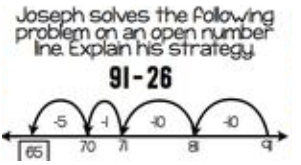
\includegraphics[width=1\linewidth]{images/numberline-add-sub-1a.png}
\end{sbspanel}%
\end{sidebyside}%
%
\item{}\begin{sidebyside}{1}{0.15}{0.15}{0}%
\begin{sbspanel}{0.7}%
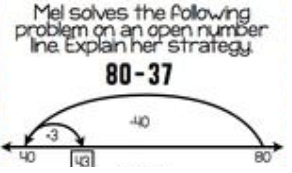
\includegraphics[width=1\linewidth]{images/numberline-add-sub-1b.png}
\end{sbspanel}%
\end{sidebyside}%
%
\end{enumerate}
\end{divisionexercise}%
\begin{divisionexercise}{2}{}{0.1}{g:exercise:idm35302782816}%
For each of the following, find the missing number by using an open number line (similar to those above).  Show at least two different methods for calculating the missing number on two different number lines.%
%
\begin{enumerate}[label=(\alph*)]
\item{}\(42+?=91 \)%
\item{}\(57+?=83 \)%
\end{enumerate}
\end{divisionexercise}%
\begin{divisionexercise}{3}{}{0.1}{g:exercise:idm35302855648}%
For the subtraction question \(53-8\), Delia, a second grade student, has done the following work:%
\begin{equation*}
53- 3=50-5=45
\end{equation*}
%
%
\begin{enumerate}[label=(\alph*)]
\item{}Explain how Delia came up with the numbers 3 and 5.%
\item{}Discuss Delia's method and answer to provide feedback.%
\item{}Use her method to answer the subtraction problem:%
\begin{equation*}
317-28
\end{equation*}
%
\end{enumerate}
\end{divisionexercise}%
\end{worksheet-section-numberless}
\restoregeometry
%
%
\typeout{************************************************}
\typeout{Worksheet 0 Decimal Addition and Subtraction with Manipulatives}
\typeout{************************************************}
%
\newgeometry{left=1.25cm, right=1.25cm, top=1.25cm, bottom=1.25cm}
\begin{worksheet-section-numberless}{Decimal Addition and Subtraction with Manipulatives}{}{Decimal Addition and Subtraction with Manipulatives}{}{}{x:worksheet:ws-decimals-add-sub}
\begin{divisionexercise}{1}{}{0.1}{g:exercise:idm35284441712}%
Show how to represent 73.2 using base blocks.  What block is worth 1 here?%
\end{divisionexercise}%
\begin{divisionexercise}{2}{}{0.1}{g:exercise:idm35284432720}%
Show how to represent 34.16 using base blocks.  What block is worth 1 here?%
\end{divisionexercise}%
\begin{divisionexercise}{3}{}{0.1}{g:exercise:idm35284453696}%
Show how to use base blocks to model%
\begin{equation*}
23.25+2.9\text{.}
\end{equation*}
Be sure to connect this to the way that we add in the standard algorithm.  What is the importance of lining up the decimal points when we add with the standard algorithm?%
\end{divisionexercise}%
\begin{divisionexercise}{4}{}{0.1}{g:exercise:idm35284506128}%
Ellie solves the subtraction problem%
\begin{equation*}
2.5-0.13
\end{equation*}
with toothpicks.  She represents 2.5 with 2 bundles of 10 toothpicks and 5 individual toothpicks.  She represents 0.13 with 1 bundle of 10 toothpicks and 3 individual toothpicks.  Ellie gets the answer 1.2.  Is she correct?  Explain.%
\end{divisionexercise}%
\end{worksheet-section-numberless}
\restoregeometry
%
%
\typeout{************************************************}
\typeout{Worksheet 0 Addition and Subtraction Problems with Strip (Tape) Diagrams}
\typeout{************************************************}
%
\newgeometry{left=1.25cm, right=1.25cm, top=1.25cm, bottom=1.25cm}
\begin{worksheet-section-numberless}{Addition and Subtraction Problems with Strip (Tape) Diagrams}{}{Addition and Subtraction Problems with Strip (Tape) Diagrams}{}{}{x:worksheet:ws-add-sub-strip-diagrams}
\begin{introduction}{}%
Directions: For each problem create strip (tape) diagram(s) to model the situation.  Also write an equation that models the situation.  Be sure that your equation matches the actual actions in the story problem, not just how you’d solve it.%
\end{introduction}%
\begin{divisionexercise}{1}{}{0.1}{g:exercise:idm35303125792}%
Rachel had 17 CDs.  After she got some more CDs, she had 43 CDs.  How many CDs did Rachel get?%
\end{divisionexercise}%
\begin{divisionexercise}{2}{}{0.1}{g:exercise:idm35303173616}%
Rachel had 43 CDs.  After she gave some away, she had 17 CDs left.  How many did she give away?%
\end{divisionexercise}%
\begin{divisionexercise}{3}{}{0.1}{g:exercise:idm35303205072}%
Rachel had some CDs.  After she gave 26 away, she had 17 left.  How many CDs did Rachel have at the start?%
\end{divisionexercise}%
\begin{divisionexercise}{4}{}{0.1}{g:exercise:idm35303267792}%
Rachel has 43 CDs.  If 26 are hip hop and the rest are rap, how many rap CDs does she have?%
\end{divisionexercise}%
\begin{divisionexercise}{5}{}{0.1}{g:exercise:idm35303290064}%
Rachel has 43 CDs.  Benny has 26 CDs.  How many more CDs does Rachel have than Benny?%
\end{divisionexercise}%
\begin{divisionexercise}{6}{}{0.1}{g:exercise:idm35303350880}%
Benny has 26 CDs. Benny has 17 fewer CDs than Rachel.  How many CDs does Rachel have?%
\end{divisionexercise}%
\begin{divisionexercise}{7}{}{0.1}{g:exercise:idm35304468272}%
Rachel has 43 CDs. Rachel has 17 more CDs than Benny.  How many CDs does Benny have?%
\end{divisionexercise}%
\end{worksheet-section-numberless}
\restoregeometry
%
%
\typeout{************************************************}
\typeout{Worksheet 0 Reasoning with Addition and Subtraction Scenarios}
\typeout{************************************************}
%
\newgeometry{left=1.25cm, right=1.25cm, top=1.25cm, bottom=1.25cm}
\begin{worksheet-section-numberless}{Reasoning with Addition and Subtraction Scenarios}{}{Reasoning with Addition and Subtraction Scenarios}{}{}{x:worksheet:ws-add-sub-reasoning}
\begin{divisionexercise}{1}{}{0.1}{g:exercise:idm35304563776}%
1.	John and Anne want to calculate \textdollar{}37-\textdollar{}19 by first calculating%
\begin{equation*}
\$37-\$20=\$17 
\end{equation*}
John says they must now subtract the \textdollar{}1 remaining from \textdollar{}17, while Anne says they must add it.  Who is correct?  Use two different models (e.g., number line and strip diagram) to represent this scenario to make it clear who is correct.%
\end{divisionexercise}%
\begin{divisionexercise}{2}{}{0.1}{g:exercise:idm35304580240}%
John and Anne want to calculate \textdollar{}3.94 -\textdollar{}1.97 by first calculating%
\begin{equation*}
\$3.97-\$1.97 = \$2 
\end{equation*}
John says in this case they also need to subtract the \textdollar{}0.03 remaining from \textdollar{}2, while Anne says they must add it.  Who is correct?  Use two different models (e.g., number line and strip diagram) to represent this scenario to make it clear who is correct.%
\end{divisionexercise}%
\begin{divisionexercise}{3}{}{0.1}{g:exercise:idm35304622560}%
Jamirez says he can calculate \textdollar{}3.74 -\textdollar{}1.97 by first adding \textdollar{}0.03 to each number and calculating \textdollar{}3.77-\textdollar{}2 instead.  How could we use a model\slash{}diagram to show that Jamirez’s method is also valid?%
\end{divisionexercise}%
\begin{divisionexercise}{4}{}{0.1}{g:exercise:idm35304644368}%
Jon’s time for running a lap in gym class is 1.4 minutes.  Jacky’s time is 1.32 minutes.  Jon thinks that he’s faster than Jacky since 4 is less than 32 so 1.4 must be less than 1.32.  Is Jon correct?  How we could convince the students whose time is faster and by how much?%
\end{divisionexercise}%
\begin{divisionexercise}{5}{}{0.1}{g:exercise:idm35304668608}%
A local park’s program committee is raising money by holding mountain bike races on a course through the local park.  During each race, a computer tracks the competitors’ locations on the course using GPS tracking.  The table below shows how far each competitor is from a checkpoint.%
\begin{sidebyside}{1}{0.05}{0.05}{0}%
\begin{sbspanel}{0.9}%
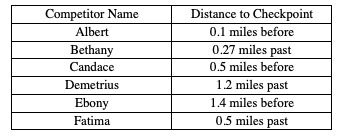
\includegraphics[width=1\linewidth]{images/reasoning-table-checkpoint.png}
\end{sbspanel}%
\end{sidebyside}%
%
\begin{enumerate}[label=(\alph*)]
\item{}The checkpoint is represented by 0 on the number line below.  Locate and label points on the number line for the positions of each listed participant. \begin{sidebyside}{1}{0.05}{0.05}{0}%
\begin{sbspanel}{0.9}%
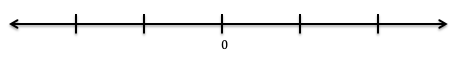
\includegraphics[width=1\linewidth]{images/blank-number-line.png}
\end{sbspanel}%
\end{sidebyside}%
%
\item{}Which competitor is closest to the checkpoint?%
\item{}Two competitors are the same distance from the checkpoint.  Are they in the same location?  Explain.%
\item{}Who is closer to finishing the race – Bethany or Candace?%
\end{enumerate}
\end{divisionexercise}%
\clearpage
\begin{divisionexercise}{6}{}{0.1}{g:exercise:idm35304749552}%
Andrea and Marta are testing three different coolers to see which keeps the temperature the coolest.  They placed a bag of ice in each cooler, and then measured the air temperature inside each cooler after 90 minutes.  The temperatures are recorded below:%
\begin{image}{0}{1}{0}%
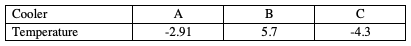
\includegraphics[width=1\linewidth]{images/reasoning-table-cooler.png}
\end{image}%
Marta wrote the following inequality: -4.3 \textless{}  -2.91 \textless{} 5.7 Andrea said Marta made a mistake, and that the inequality should be: -2.91 \textless{} -4.3 \textless{} 5.7%
\par
Is either student correct?  Explain.  Use a number line to help justify your answer.  What misconceptions might the student(s) have had that caused the incorrect inequality?%
\end{divisionexercise}%
\end{worksheet-section-numberless}
\restoregeometry
%
%
\typeout{************************************************}
\typeout{Worksheet 0 Exploring Fractions-{}-{}Rectangle (Area) Model Representation}
\typeout{************************************************}
%
\newgeometry{left=1.25cm, right=1.25cm, top=1.25cm, bottom=1.25cm}
\begin{worksheet-section-numberless}{Exploring Fractions-{}-{}Rectangle (Area) Model Representation}{}{Exploring Fractions-{}-{}Rectangle (Area) Model Representation}{}{}{x:worksheet:ws-fractions-intro-rectangle}
\begin{introduction}{}%
For each problem, keep in mind how you might explain your process.%
\end{introduction}%
\begin{divisionexercise}{1}{}{0.1}{g:exercise:idm35303060608}%
If the following rectangle is one whole, show two-thirds. \begin{sidebyside}{1}{0.3}{0.3}{0}%
\begin{sbspanel}{0.4}%
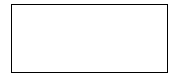
\includegraphics[width=1\linewidth]{images/generic-rectangle.png}
\end{sbspanel}%
\end{sidebyside}%
%
\end{divisionexercise}%
\begin{divisionexercise}{2}{}{0.1}{g:exercise:idm35304837872}%
If the following rectangle is one whole, show five-thirds. \begin{sidebyside}{1}{0.3}{0.3}{0}%
\begin{sbspanel}{0.4}%
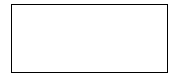
\includegraphics[width=1\linewidth]{images/generic-rectangle.png}
\end{sbspanel}%
\end{sidebyside}%
%
\end{divisionexercise}%
\begin{divisionexercise}{3}{}{0.1}{g:exercise:idm35304864640}%
If the following rectangle is three-fourths, draw one whole. \begin{sidebyside}{1}{0.35}{0.35}{0}%
\begin{sbspanel}{0.3}%
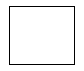
\includegraphics[width=1\linewidth]{images/generic-square.png}
\end{sbspanel}%
\end{sidebyside}%
%
\end{divisionexercise}%
\clearpage
\begin{divisionexercise}{4}{}{0.1}{g:exercise:idm35304907776}%
If this rectangle is four-thirds, show what rectangle could be the whole. \begin{sidebyside}{1}{0.3}{0.3}{0}%
\begin{sbspanel}{0.4}%
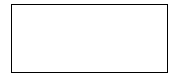
\includegraphics[width=1\linewidth]{images/generic-rectangle.png}
\end{sbspanel}%
\end{sidebyside}%
%
\end{divisionexercise}%
\begin{divisionexercise}{5}{}{0.1}{g:exercise:idm35304938960}%
Maria says that the shaded region below represents the fraction \(\frac{9}{12} \). Carmina says the shaded region represents the fraction \(\frac{9}{4} \). Explain why each of the two student’s answers can be considered correct. \begin{sidebyside}{1}{0.25}{0.25}{0}%
\begin{sbspanel}{0.5}%
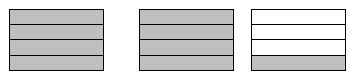
\includegraphics[width=1\linewidth]{images/nine-fourths-vs-twelfths.png}
\end{sbspanel}%
\end{sidebyside}%
%
\end{divisionexercise}%
\end{worksheet-section-numberless}
\restoregeometry
%
%
\typeout{************************************************}
\typeout{Worksheet 0 Exploring Fractions-{}-{}Set Model Representation}
\typeout{************************************************}
%
\newgeometry{left=1.25cm, right=1.25cm, top=1.25cm, bottom=1.25cm}
\begin{worksheet-section-numberless}{Exploring Fractions-{}-{}Set Model Representation}{}{Exploring Fractions-{}-{}Set Model Representation}{}{}{x:worksheet:ws-fractions-intro-sets}
\begin{divisionexercise}{1}{}{0.1}{g:exercise:idm35304509872}%
If 14 counters are one whole, shade the counters that make three-sevenths. \begin{sidebyside}{1}{0.35}{0.35}{0}%
\begin{sbspanel}{0.3}%
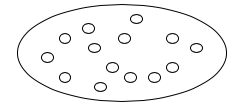
\includegraphics[width=1\linewidth]{images/fourteen-counters.png}
\end{sbspanel}%
\end{sidebyside}%
%
\end{divisionexercise}%
\begin{divisionexercise}{2}{}{0.1}{g:exercise:idm35304539264}%
Draw 12 counters like \#1. If 12 counters are one whole, how many are in five-thirds of a set?%
\end{divisionexercise}%
\begin{divisionexercise}{3}{}{0.1}{g:exercise:idm35304979904}%
Draw 21 coutners. If 21 counters are three-fifths of a set, how many counters are in the full set (1 whole)?%
\end{divisionexercise}%
\begin{divisionexercise}{4}{}{0.1}{g:exercise:idm35305030048}%
Draw 12 counters. If 12 counters are three-halves of a set, how many counters are in one set (1 whole)?%
\end{divisionexercise}%
\begin{divisionexercise}{5}{}{}{g:exercise:idm35305052256}%
What fraction of this set is shaded in? \begin{sidebyside}{1}{0.35}{0.35}{0}%
\begin{sbspanel}{0.3}%
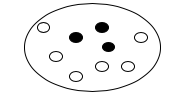
\includegraphics[width=1\linewidth]{images/counters-one-third.png}
\end{sbspanel}%
\end{sidebyside}%
%
\end{divisionexercise}%
\end{worksheet-section-numberless}
\restoregeometry
%
%
\typeout{************************************************}
\typeout{Worksheet 0 Exploring Fractions-{}-{}Cuisenaire Rods}
\typeout{************************************************}
%
\newgeometry{left=1.25cm, right=1.25cm, top=1.25cm, bottom=1.25cm}
\begin{worksheet-section-numberless}{Exploring Fractions-{}-{}Cuisenaire Rods}{}{Exploring Fractions-{}-{}Cuisenaire Rods}{}{}{x:worksheet:ws-fractions-intro-Cuisenaire}
\begin{introduction}{}%
For Online Cuisenaire Rods, go to: http:\slash{}\slash{}\slash{}nrich.maths.org\slash{}4348%
\end{introduction}%
\begin{divisionexercise}{1}{}{0.1}{g:exercise:idm35305123040}%
Select a brown Cuisenaire Rod.  If brown is the whole, which rod is one-fourth?%
\end{divisionexercise}%
\begin{divisionexercise}{2}{}{0.1}{g:exercise:idm35305147408}%
If dark green is the whole, what rod represents two-thirds? What rod represents three-halves?%
\end{divisionexercise}%
\begin{divisionexercise}{3}{}{0.1}{g:exercise:idm35305167792}%
Select a dark green Cuisenaire Rod.  If dark green is two-thirds, what rod is the whole?%
\end{divisionexercise}%
\begin{divisionexercise}{4}{}{0.1}{g:exercise:idm35305179152}%
Select a yellow Cuisenaire Rod.  If yellow is five-fourths, what rod is one whole? What rod is 2?%
\end{divisionexercise}%
\begin{divisionexercise}{5}{}{0.1}{g:exercise:idm35305190864}%
Select a dark green Cuisenaire Rod.  If dark green is the whole, what fraction is the yellow rod?%
\end{divisionexercise}%
\begin{divisionexercise}{6}{}{0.1}{g:exercise:idm35305201248}%
If the brown rod is one whole, what fraction is the orange rod?%
\end{divisionexercise}%
\begin{divisionexercise}{7}{}{0.1}{g:exercise:idm35305211312}%
If the blue rod is 3, what rod represents \(\frac{2}{3} \)?%
\end{divisionexercise}%
\end{worksheet-section-numberless}
\restoregeometry
%
%
\typeout{************************************************}
\typeout{Worksheet 0 Exploring Fractions-{}-{}Pattern Blocks Representation}
\typeout{************************************************}
%
\newgeometry{left=1.25cm, right=1.25cm, top=1.25cm, bottom=1.25cm}
\begin{worksheet-section-numberless}{Exploring Fractions-{}-{}Pattern Blocks Representation}{}{Exploring Fractions-{}-{}Pattern Blocks Representation}{}{}{x:worksheet:ws-fractions-intro-patternblocks}
\begin{introduction}{}%
Pattern blocks include the yellow hexagon, blue parallelogram, red trapezoid, and green triangle. For Online Pattern Blocks, go to: http:\slash{}\slash{}www.mathplayground.com\slash{}patternblocks.html)%
\end{introduction}%
\begin{introduction}{}%
If the yellow hexagon represents one whole:%
\end{introduction}%
\begin{divisionexercise}{1}{}{0.1}{g:exercise:idm35305298176}%
What shape would represent \(\frac{1}{2} \) ?%
\end{divisionexercise}%
\begin{divisionexercise}{2}{}{0.1}{g:exercise:idm35305310192}%
What shape would represent \(\frac{1}{3} \) ?%
\end{divisionexercise}%
\begin{divisionexercise}{3}{}{0.1}{g:exercise:idm35305327744}%
What shape would represent \(\frac{1}{6} \)?%
\end{divisionexercise}%
\begin{introduction}{}%
If the blue parallelogram represents one whole:%
\end{introduction}%
\begin{divisionexercise}{4}{}{0.1}{g:exercise:idm35305341824}%
What fraction would the red trapezoid represent?%
\end{divisionexercise}%
\begin{divisionexercise}{5}{}{0.1}{g:exercise:idm35305354576}%
What fraction would the green triangle represent?%
\end{divisionexercise}%
\clearpage
\begin{divisionexercise}{6}{}{0.1}{g:exercise:idm35305373696}%
What fraction would the yellow hexagon represent?%
\end{divisionexercise}%
\begin{introduction}{}%
If the double hexagon represents one whole:%
\end{introduction}%
\begin{divisionexercise}{7}{}{0.1}{g:exercise:idm35305402048}%
What fraction would the red trapezoid represent?%
\end{divisionexercise}%
\begin{divisionexercise}{8}{}{0.1}{g:exercise:idm35305417808}%
What fraction would the green triangle represent?%
\end{divisionexercise}%
\begin{divisionexercise}{9}{}{0.1}{g:exercise:idm35305433520}%
What fraction would the yellow hexagon represent?%
\end{divisionexercise}%
\begin{divisionexercise}{10}{}{0.1}{g:exercise:idm35305442432}%
If the red trapezoid equals \(\frac{3}{5} \), what shape or shapes, when combined, could represent 1?  How many different shape combinations are there?%
\end{divisionexercise}%
\end{worksheet-section-numberless}
\restoregeometry
%
%
\typeout{************************************************}
\typeout{Worksheet 0 Exploring Fractions-{}-{}Number Line Representation}
\typeout{************************************************}
%
\newgeometry{left=1.25cm, right=1.25cm, top=1.25cm, bottom=1.25cm}
\begin{worksheet-section-numberless}{Exploring Fractions-{}-{}Number Line Representation}{}{Exploring Fractions-{}-{}Number Line Representation}{}{}{x:worksheet:ws-fractions-intro-numberline}
\begin{divisionexercise}{1}{}{0.1}{g:exercise:idm35305225696}%
On the number line below, \(a= 0 \) and \(b=1 \).  Use the meaning of fractions to plot three-fifths.%
\begin{sidebyside}{1}{0}{0}{0}%
\begin{sbspanel}{1}%
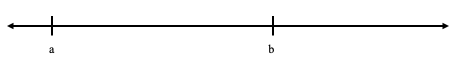
\includegraphics[width=1\linewidth]{images/fractions-number-line.png}
\end{sbspanel}%
\end{sidebyside}%
\end{divisionexercise}%
\begin{divisionexercise}{2}{}{0.1}{g:exercise:idm35304497872}%
On the number line below, \(a= 0 \) and \(b=\frac{6}{5} \).  Use the meaning of fractions to plot one-whole (1).%
\begin{sidebyside}{1}{0}{0}{0}%
\begin{sbspanel}{1}%
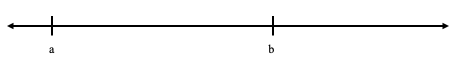
\includegraphics[width=1\linewidth]{images/fractions-number-line.png}
\end{sbspanel}%
\end{sidebyside}%
\end{divisionexercise}%
\end{worksheet-section-numberless}
\restoregeometry
%
%
\typeout{************************************************}
\typeout{Worksheet 0 Equivalent Fractions}
\typeout{************************************************}
%
\newgeometry{left=1.25cm, right=1.25cm, top=1.25cm, bottom=1.25cm}
\begin{worksheet-section-numberless}{Equivalent Fractions}{}{Equivalent Fractions}{}{}{x:worksheet:ws-equiv-fractions}
\begin{divisionexercise}{1}{}{0.4}{g:exercise:idm35305461456}%
Discrete Models: Choose 18 counters as the whole. In the space below, describe how you might convince a student that two-thirds, four-sixths, and six-ninths are equivalent fractions.%
\end{divisionexercise}%
\begin{divisionexercise}{2}{}{0.4}{g:exercise:idm35305469104}%
Now, represent \(\frac{2}{3} \) using a fraction bar (tape diagram). Then, show  \(\frac{2 \times 2}{3 \times 2} \) on the model. What is the answer? In your picture, where do we see multiplying the numerator and denominator by 2? Be very specific!!!%
\end{divisionexercise}%
\begin{divisionexercise}{3}{}{0.2}{g:exercise:idm35305488016}%
Now, represent represent \(\frac{4}{10} \) using a fraction bar (tape diagram). Then, show  \(\frac{4 \div 2}{10 \div 2} \) on the model. What is the answer? In your picture, where do we see dividing the numerator and denominator by 2? Be very specific!!!!%
\end{divisionexercise}%
\begin{introduction}{}%
For each of the following problems use one of the models (area model, set model (chips), rods, pattern blocks, fraction bars, fraction circles) to represent your solution process.%
\end{introduction}%
\begin{divisionexercise}{4}{}{0.2}{g:exercise:idm35279105280}%
Jean has a casserole recipe that calls for \(\frac{1}{2} \) cup of butter. Jean only has \(\frac{1}{3} \) cup of butter. Assuming that Jean has enough of the other ingredients what fractions of the casserole recipe can Jean make? Make math drawings or use manipulatives to help you solve this problem. Explain why your answer is correct. In your explanation, attend carefully to the whole (unit amount) that each fraction is of.%
\end{divisionexercise}%
\begin{divisionexercise}{5}{}{0}{g:exercise:idm35279145200}%
One serving of SnackOs is \(\frac{2}{3} \) of a cup. Jane wants to eat \(\frac{1}{3} \) of a serving of SnackOs. What fraction of a cup of SnackOs should Jane eat? Make math drawings to help you solve this problem. Explain why your answer is correct. In your explanation, attend carefully to the whole (unit amount) that each fraction is of.%
\end{divisionexercise}%
\end{worksheet-section-numberless}
\restoregeometry
%
%
\typeout{************************************************}
\typeout{Worksheet 0 Comparing Fractions}
\typeout{************************************************}
%
\newgeometry{left=1.25cm, right=1.25cm, top=1.25cm, bottom=1.25cm}
\begin{worksheet-section-numberless}{Comparing Fractions}{}{Comparing Fractions}{}{}{x:worksheet:ws-comparing-fractions}
\begin{introduction}{}%
At a birthday party everyone is about to sit down for pizza.  All the pizzas in this problem are the same size, and the same toppings are distributed evenly on all pizzas.%
\end{introduction}%
\begin{divisionexercise}{1}{}{0.1}{g:exercise:idm35302537344}%
At one table there are 4 pizzas and 8 chairs.  At the other table there are 4 pizzas and 10 chairs.  Carlos knows that everyone at the party is pretty hungry, and assumes that the pizzas at each table will be split evenly, so he wants to sit at the table at which he will end up with the most pizza.  Which table should he choose?  Assume that the pizzas are uncut until all chairs at the table are occupied.%
\end{divisionexercise}%
\begin{divisionexercise}{2}{}{0.1}{g:exercise:idm35302584304}%
What if, at one table there are 3 pizzas and 8 chairs, and at the other table there are 4 pizzas and 10 chairs.  Carlos, again, knows that everyone at the party is pretty hungry, and assumes that the pizzas at each table will be split evenly.  He still wants to sit at the table at which he will end up with the most pizza.  Which table should he choose in this situation? Assume that the pizzas are uncut until all chairs at the table are occupied.%
\end{divisionexercise}%
\begin{divisionexercise}{3}{}{0.1}{g:exercise:idm35302651952}%
Which fraction in each pair is greater?  Give one or more reasons.  Do NOT use drawings, models, common denominators, or cross-multiplication.  Rely on your existing knowledge about the size of various fractions and\slash{}or the size of the pieces in different fractions, e.g., compare to benchmark numbers like 0, \(\frac{1}{2} \) and 1, or make comparisons based on the size of the pieces.%
%
\begin{enumerate}[label=(\alph*)]
\item{}\(\frac{4}{5} \) or \(\frac{4}{9} \)%
\item{}\(\frac{5}{3} \) or \(\frac{5}{8} \)%
\item{}\(\frac{5}{8} \) or \(\frac{7}{12} \)%
\item{}\(\frac{3}{4} \) or \(\frac{9}{10} \)%
\end{enumerate}
\end{divisionexercise}%
\clearpage
\begin{divisionexercise}{4}{}{0.3}{g:exercise:idm35303098736}%
Find two fractions between each pair of fractions given below. Plot all four fractions on a number line.%
%
\begin{enumerate}[label=(\alph*)]
\item{}\(\frac{2}{5} \) and \(\frac{3}{5} \)%
\item{}\(\frac{2}{3} \) and \(\frac{3}{5} \)%
\end{enumerate}
\end{divisionexercise}%
\begin{divisionexercise}{5}{}{}{g:exercise:idm35304529664}%
Without using a calculator, mark where each of the following fractions belongs on the following number line. Describe how you determined where to place each fraction.%
\par
%
\begin{equation*}
\frac{5}{12} , \frac{4}{7} , \frac{3}{7} , \frac{3}{8} , \frac{2}{3} , \frac{6}{7} 
\end{equation*}
%
\begin{sidebyside}{1}{0.05}{0.05}{0}%
\begin{sbspanel}{0.9}%
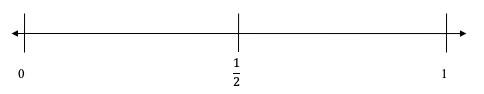
\includegraphics[width=1\linewidth]{images/number-line-half-one.png}
\end{sbspanel}%
\end{sidebyside}%
\end{divisionexercise}%
\end{worksheet-section-numberless}
\restoregeometry
%
%
\typeout{************************************************}
\typeout{Worksheet 0 Pizza Splitting Problem, Part 2}
\typeout{************************************************}
%
\newgeometry{left=1.25cm, right=1.25cm, top=1.25cm, bottom=1.25cm}
\begin{worksheet-section-numberless}{Pizza Splitting Problem, Part 2}{}{Pizza Splitting Problem, Part 2}{}{}{x:worksheet:ws-pizza-splitting-problem}
\begin{divisionexercise}{1}{}{0.2}{g:exercise:idm35305257584}%
Now, assume that each pizza is already cut into 12 equal pieces. At one table there are 3 pizzas and 8 chairs.  At the other table there are 4 pizzas and 10 chairs.  Which table should he choose?%
\end{divisionexercise}%
\begin{divisionexercise}{2}{}{0.2}{g:exercise:idm35305272544}%
Suppose now that, instead of dividing up the pizza separately at each table, the hosts decide to give all 18 people equal amounts from the 7 pizzas.  Carlos realizes that this means that the amount everyone ends up with is in between the amounts they would have ended up with if each pizza had only been shared among those at the same table.  How can we state this observation in terms of fractions?  How can we state this observation in terms of straight-line graphs?  Is there a general relationship about fractions that this is illustrating?  Is there a general graphical relationship that this is illustrating?%
\end{divisionexercise}%
\clearpage
\begin{divisionexercise}{3}{}{0.1}{g:exercise:idm35305097248}%
Maria solved problem 2 on handout 1 by using graph paper and drawing two straight lines.  She is wondering what the lines represent, what their equations are and what other problems could be solved with them, now that the lines are drawn.  She is also wondering what the slope of each line represents.  What can we tell Maria on these questions?%
\begin{sidebyside}{1}{0.05}{0.05}{0}%
\begin{sbspanel}{0.9}%
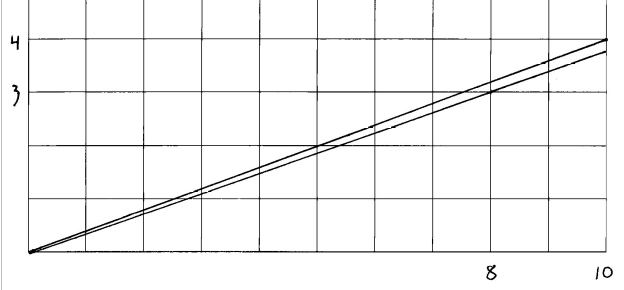
\includegraphics[width=1\linewidth]{images/pizza-splitting-problem.png}
\end{sbspanel}%
\end{sidebyside}%
\end{divisionexercise}%
\begin{divisionexercise}{4}{}{0.1}{g:exercise:idm35284428768}%
(Refer to Problem 2 on Comparing Fractions Worksheet) At one table there are 3 pizzas and 8 chairs, and at the other table there are 4 pizzas and 10 chairs.  Carlos, again, knows that everyone at the party is pretty hungry, and assumes that the pizzas at each table will be split evenly, he still wants to sit at the table at which he will end up with the most pizza.  Which table should he choose in this situation? Assume that the pizzas are uncut until all chairs at the table are occupied.%
\end{divisionexercise}%
\begin{divisionexercise}{5}{}{0.1}{g:exercise:idm35304922880}%
Create and interpret a double number line way to solve this problem.%
\end{divisionexercise}%
\begin{divisionexercise}{6}{}{}{g:exercise:idm35304835488}%
On Graph paper, create and interpret a People vs Pizza graph to solve this problem, and relate it to the previous double number line.%
\end{divisionexercise}%
\end{worksheet-section-numberless}
\restoregeometry
%
%
\typeout{************************************************}
\typeout{Worksheet 0 Addition and Subtraction of Fractions}
\typeout{************************************************}
%
\newgeometry{left=1.25cm, right=1.25cm, top=1.25cm, bottom=1.25cm}
\begin{worksheet-section-numberless}{Addition and Subtraction of Fractions}{}{Addition and Subtraction of Fractions}{}{}{x:worksheet:ws-add-sub-fractions}
\begin{introduction}{}%
Use one of the concrete models (fraction bars or circles or pattern blocks or chip model) to solve the following problems. Discuss the importance of the whole and the meaning of finding common denominators.%
\end{introduction}%
\begin{divisionexercise}{1}{}{0.2}{g:exercise:idm35305180944}%
\(\frac{1}{3} + \frac{1}{2} \)%
\end{divisionexercise}%
\begin{divisionexercise}{2}{}{0.2}{g:exercise:idm35305224320}%
\(\frac{5}{6} - \frac{1}{4} \)%
\end{divisionexercise}%
\begin{divisionexercise}{3}{}{0.2}{g:exercise:idm35305313088}%
\(\frac{2}{3} + \frac{3}{4} \)%
\end{divisionexercise}%
\clearpage
\begin{divisionexercise}{4}{}{0.1}{g:exercise:idm35305334624}%
Use a rectangle model (area model) to find the sum and the difference of \(\frac{1}{3} \) and \(\frac{1}{4} \).  Discuss why we need to find common denominators, how a common denominator is reflected in the area model and “equal parts” are represented in the picture.%
\end{divisionexercise}%
\begin{introduction}{}%
Practice using the rectangle model with the following questions.%
\end{introduction}%
\begin{divisionexercise}{5}{}{0.2}{g:exercise:idm35305384032}%
\(\frac{2}{5} + \frac{1}{3} \)%
\end{divisionexercise}%
\begin{divisionexercise}{6}{}{0.2}{g:exercise:idm35305425888}%
\(\frac{3}{4} + \frac{5}{6} \)%
\end{divisionexercise}%
\begin{divisionexercise}{7}{}{0.2}{g:exercise:idm35305462656}%
\(\frac{3}{5} - \frac{1}{4}  \)%
\end{divisionexercise}%
\begin{divisionexercise}{8}{}{0.2}{g:exercise:idm35279601824}%
\(\frac{5}{6} - \frac{1}{4} \)%
\end{divisionexercise}%
\end{worksheet-section-numberless}
\restoregeometry
%
%
\typeout{************************************************}
\typeout{Worksheet 0 Egyptian Fractions}
\typeout{************************************************}
%
\newgeometry{left=1.25cm, right=1.25cm, top=1.25cm, bottom=1.25cm}
\begin{worksheet-section-numberless}{Egyptian Fractions}{}{Egyptian Fractions}{}{}{x:worksheet:ws-add-sub-fractions-extension}
\begin{introduction}{}%
The ancient Egyptians wrote any fraction as a sum of fractions with numerators of 1 and all different denominators.  For example they would have expressed \(\frac{2}{3} \) as \(\frac{1}{2} + \frac{1}{6} \) (their notation was different than this).  Fractions expressed as a sum of fractions with numerators of 1 and denominators that are all different are often called “Egyptian Fractions” for this reason.%
\par
Find an Egyptian Fraction Representation for each of the fractions below:%
\end{introduction}%
\begin{divisionexercise}{1}{}{0.1}{g:exercise:idm35305113696}%
\(\frac{3}{4} \)%
\end{divisionexercise}%
\begin{divisionexercise}{2}{}{0.1}{g:exercise:idm35305036624}%
\(\frac{5}{6} \)%
\end{divisionexercise}%
\begin{divisionexercise}{3}{}{0.1}{g:exercise:idm35304947360}%
\(\frac{4}{5} \)%
\end{divisionexercise}%
\begin{divisionexercise}{4}{}{0.1}{g:exercise:idm35305383296}%
Explain how your answer for \(\frac{5}{6} \) might be used to help you split five loaves of bread among six people.%
\end{divisionexercise}%
\end{worksheet-section-numberless}
\restoregeometry
%
%
\typeout{************************************************}
\typeout{Worksheet 0 Integer Addition and Subtraction}
\typeout{************************************************}
%
\newgeometry{left=1.25cm, right=1.25cm, top=1.25cm, bottom=1.25cm}
\begin{worksheet-section-numberless}{Integer Addition and Subtraction}{}{Integer Addition and Subtraction}{}{}{x:worksheet:ws-add-sub-integers}
\begin{introduction}{}%
Exploration 1: Integer Addition%
\par
Use the ``Union of two Disjoint Sets'' Model for Addition to solve each of the following problems: \begin{sidebyside}{1}{0}{0}{0}%
\begin{sbspanel}{1}%
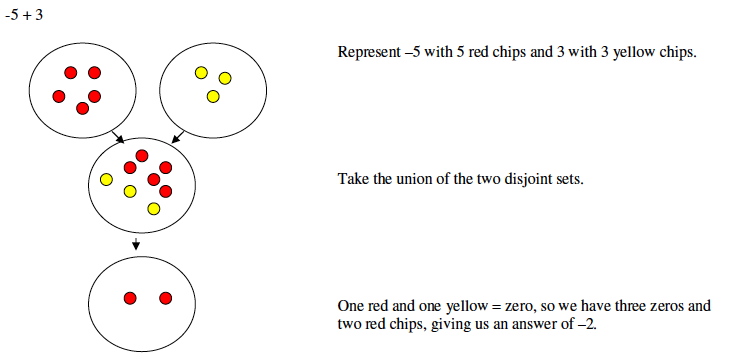
\includegraphics[width=1\linewidth]{images/integer-add-model.png}
\end{sbspanel}%
\end{sidebyside}%
%
\end{introduction}%
\begin{divisionexercise}{1}{}{0.2}{g:exercise:idm35279799024}%
4+3%
\end{divisionexercise}%
\clearpage
\begin{divisionexercise}{2}{}{0.2}{g:exercise:idm35281152048}%
\((-3)+(-6) \)%
\end{divisionexercise}%
\begin{divisionexercise}{3}{}{0.2}{g:exercise:idm35280373040}%
\(3+(-7) \)%
\end{divisionexercise}%
\begin{divisionexercise}{4}{}{0.2}{g:exercise:idm35281013008}%
\((-8)+ 5 \)%
\end{divisionexercise}%
\clearpage
\begin{introduction}{}%
Exploration 2: Integer Subtraction%
\par
Use the ``Take-Away Set'' Model for Subtraction to solve each of the following problems: \begin{sidebyside}{1}{0}{0}{0}%
\begin{sbspanel}{1}%
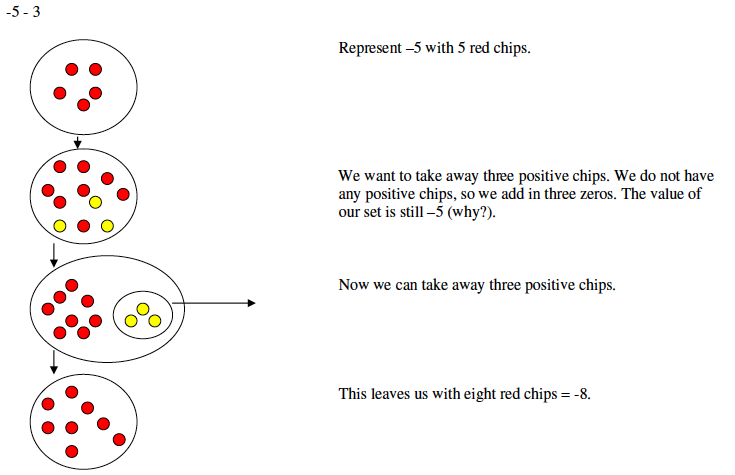
\includegraphics[width=1\linewidth]{images/integer-sub-model.png}
\end{sbspanel}%
\end{sidebyside}%
%
\end{introduction}%
\begin{divisionexercise}{5}{}{0.3}{g:exercise:idm35279962672}%
5-9%
\end{divisionexercise}%
\clearpage
\begin{divisionexercise}{6}{}{0.2}{g:exercise:idm35280923088}%
\((-6)-(-5) \)%
\end{divisionexercise}%
\begin{divisionexercise}{7}{}{0.2}{g:exercise:idm35280960096}%
\(3-(-4) \)%
\end{divisionexercise}%
\begin{divisionexercise}{8}{}{0.2}{g:exercise:idm35302588368}%
\((-4)-(-8) \)%
\end{divisionexercise}%
\end{worksheet-section-numberless}
\restoregeometry
%
%
\typeout{************************************************}
\typeout{Worksheet 0 Integer Arithmetic Situations}
\typeout{************************************************}
%
\newgeometry{left=1.25cm, right=1.25cm, top=1.25cm, bottom=1.25cm}
\begin{worksheet-section-numberless}{Integer Arithmetic Situations}{}{Integer Arithmetic Situations}{}{}{x:worksheet:ws-integer-arithmetic-situations}
\begin{introduction}{}%
The set of numbers called the integers is a subset of the real numbers (any number that can be found on the number line).  The set is comprised of positive integers (1, 2, 3, 4, etc.), negative integers (-1, -2, -3, -4, etc.), and 0, which is neither positive nor negative.  Use your knowledge of integers and their opposites to complete this activity.%
\end{introduction}%
\begin{divisionexercise}{1}{}{0.3}{g:exercise:idm35304962976}%
Investigate what happens when you calculate ``6-3'';  ``6-2'';  ``6-1'' ;``6-0''; ``6-(-1)'';     ``6-(-2)''; ``6-(-3)''.  Explain why it makes sense that 6- (-3) = 6+3 = 9.   Refer to a pattern you notice in your calculation.%
\end{divisionexercise}%
\begin{introduction}{}%
Solve the following temperature model problems using a picture.%
\end{introduction}%
\begin{divisionexercise}{2}{}{0.2}{g:exercise:idm35279191952}%
It was -3 degrees C at dawn. In the meantime, the temperature went up 5 degrees C. Now what is the temperature?%
\end{divisionexercise}%
\clearpage
\begin{divisionexercise}{3}{}{0.2}{g:exercise:idm35279206336}%
The temperature was 5 degrees C in Greeley. At the same time it was -3 degrees C in Denver. How much warmer was it in Greeley than in Denver?%
\end{divisionexercise}%
\begin{divisionexercise}{4}{}{0.2}{g:exercise:idm35279892032}%
The temperature during the day was -3 degrees C in Greeley and it dropped 2 degrees C more by midnight. What was the temperature at midnight?%
\end{divisionexercise}%
\begin{divisionexercise}{5}{}{0.2}{g:exercise:idm35305423040}%
The top of Mount Everest is at an elevation of 29029 feet above sea level, and the deepest part of the ocean in the Mariana Trench is 36070 feet below sea level.  How much higher is the top of Mount Everest compared to the lowest point in the ocean?%
\end{divisionexercise}%
\clearpage
\begin{divisionexercise}{6}{}{0.2}{g:exercise:idm35280144400}%
Write integer addition and subtraction equations that are naturally suggested by problems 4 and 5 and briefly discuss how these examples can help students understand addition and subtraction of positive and negative numbers.%
\end{divisionexercise}%
\end{worksheet-section-numberless}
\restoregeometry
%
%
\typeout{************************************************}
\typeout{Worksheet 0 Multiplication Models}
\typeout{************************************************}
%
\newgeometry{left=1.25cm, right=1.25cm, top=1.25cm, bottom=1.25cm}
\begin{worksheet-section-numberless}{Multiplication Models}{}{Multiplication Models}{}{}{x:worksheet:ws-multiplication-models}
\begin{introduction}{}%
Exploration \#1: Recall A \(\times \) B refers to the number of objects in A groups of B objects.  The product A \(\times \) B gives the total number of objects.  For the following story problems, write the corresponding multiplication statement and explicitly identify what are the groups, what are the objects in each group, and what does the product represent.%
\end{introduction}%
\begin{divisionexercise}{1}{}{0.1}{g:exercise:idm35280990416}%
If apples cost \textdollar{}2 per pound, how much will 5 pounds of apples cost?%
\end{divisionexercise}%
\begin{divisionexercise}{2}{}{0.1}{g:exercise:idm35281010976}%
How many hours are in a week?%
\end{divisionexercise}%
\begin{divisionexercise}{3}{}{0.1}{g:exercise:idm35281029152}%
A carpet is 4 feet long and 3 feet wide. What is its area?%
\end{divisionexercise}%
\begin{divisionexercise}{4}{}{0.1}{g:exercise:idm35281049776}%
Rémi has 4 different pairs of pants and 3 different shirts. How many different outfits consisting of a pair of pants and a shirt can Rémi make from these clothes?%
\end{divisionexercise}%
\clearpage
\begin{introduction}{}%
Exploration \#2: Each of the three models below can be used to represent the process of multiplying 4 by 3.  Discuss the following questions using these figures.%
%
\begin{description}
\item[{}]Figure 1: This could be viewed as a 2-dimensional array model or a rectangular area model. \begin{sidebyside}{1}{0.45}{0.45}{0}%
\begin{sbspanel}{0.1}%
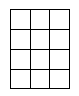
\includegraphics[width=1\linewidth]{images/mult-array.png}
\end{sbspanel}%
\end{sidebyside}%
\item[{}]Figure 2: A tree diagram \begin{sidebyside}{1}{0.45}{0.45}{0}%
\begin{sbspanel}{0.1}%
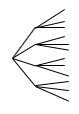
\includegraphics[width=1\linewidth]{images/mult-tree.png}
\end{sbspanel}%
\end{sidebyside}%
\item[{}]Figure 3: This could be viewed as an array model with one row only. \begin{sidebyside}{1}{0.3}{0.3}{0}%
\begin{sbspanel}{0.4}%
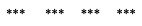
\includegraphics[width=1\linewidth]{images/mult-one-row.png}
\end{sbspanel}%
\end{sidebyside}%
\end{description}
\end{introduction}%
\begin{divisionexercise}{5}{}{0.1}{g:exercise:idm35302500480}%
Which figure can be easily associated with the ``repeated addition'' idea? Why?%
\end{divisionexercise}%
\begin{divisionexercise}{6}{}{0.1}{g:exercise:idm35305212528}%
Which picture makes it easiest to see that \(4 \times 3 = 3 \times 4 \) (commutative property of multiplication)?%
\end{divisionexercise}%
\begin{divisionexercise}{7}{}{0.1}{g:exercise:idm35280519008}%
Which picture might be most helpful if you wanted to illustrate another round of multiplication, for example 4 times 3 times 2 (and also the associative property of multiplication)?%
\end{divisionexercise}%
\clearpage
\begin{introduction}{}%
Exploration \#3: Associative and Commutative Properties of Multiplication%
\par
How can we use properties of multiplication to do the following mental math problems in our heads?%
\end{introduction}%
\begin{divisionexercise}{8}{}{0.15}{g:exercise:idm35278785824}%
\(16 \times 25  \)%
\end{divisionexercise}%
\begin{divisionexercise}{9}{}{0.15}{g:exercise:idm35278875232}%
\(5 \times 32  \)%
\end{divisionexercise}%
\begin{divisionexercise}{10}{}{0.15}{g:exercise:idm35278971280}%
\(4 \times 10 \times 7  \)%
\end{divisionexercise}%
\begin{introduction}{}%
Exploration \#4: Story Problems with Multiplication\end{introduction}%
\begin{divisionexercise}{11}{}{0.1}{g:exercise:idm35279037248}%
Dave and Roberto want to know how many one-inch-by-one-inch squares it would take to cover the floor of a room that is 10 feet by 8 feet.  They multiply 10 by 8 by 12 and decide that they would need 960 one-inch squares.  Their calculation is incorrect, explain why it is incorrect and why Dave and Roberto might be thinking this way.%
\end{divisionexercise}%
\clearpage
\begin{divisionexercise}{12}{}{0.2}{g:exercise:idm35279124704}%
In a school project students make short, pretend license plates for their model cars.  The license plates can only use the letters A, B, and C and the numbers 1 and 2.  There must be two letters followed by two numbers, and letters and numbers can be used over again.  For example, one possible license plate is AA11. Another is CA21. How many total license plates of this type can be made?%
\end{divisionexercise}%
\begin{divisionexercise}{13}{}{0.2}{g:exercise:idm35279269264}%
How many total license plates can be made using three of any letter (26 choices) followed by four digits (10 choices, 0 through 9)?  Explain by analogy using ideas from the previous two questions%
\end{divisionexercise}%
\begin{divisionexercise}{14}{}{0.2}{g:exercise:idm35279487728}%
Suppose a school club had 6 members. In how many ways can they choose the club President and Vice President? Use one of the models for multiplication discussed in Exploration \#1 to illustrate your process.%
\end{divisionexercise}%
\clearpage
\begin{divisionexercise}{15}{}{0.2}{g:exercise:idm35279831936}%
Revisit the last question: Suppose a school club had 6 members. In how many ways can they choose the co-president pair? Is your answer different than for the other question?  Explain.%
\end{divisionexercise}%
\begin{introduction}{}%
Exploration \#5: Special Case – Multiplying by 10.\end{introduction}%
\begin{divisionexercise}{16}{}{0.2}{g:exercise:idm35279924992}%
Using the example \(10 \times 32 \), explain a strategy to find the product. Using base-ten blocks show why your strategy works.%
\end{divisionexercise}%
\begin{divisionexercise}{17}{}{0.2}{g:exercise:idm35280105168}%
Does your strategy work with \(10 \times 3.2 \)? Explain and show using base 10 blocks and\slash{}or decimal squares.%
\end{divisionexercise}%
\clearpage
\begin{divisionexercise}{18}{}{0.2}{g:exercise:idm35280193184}%
Clark says \(10 \times 4.7=4.70 \). Why might Clark think this? Provide an explanation to Clark why his answer is not correct, provide the correct answer and explain how the correct answer is obtained.%
\end{divisionexercise}%
\end{worksheet-section-numberless}
\restoregeometry
%
%
\typeout{************************************************}
\typeout{Worksheet 0 Fraction Multiplication}
\typeout{************************************************}
%
\newgeometry{left=1.25cm, right=1.25cm, top=1.25cm, bottom=1.25cm}
\begin{worksheet-section-numberless}{Fraction Multiplication}{}{Fraction Multiplication}{}{}{x:worksheet:ws-mult-fractions}
\begin{introduction}{}%
Draw pictures that help us find the following products.  Make sure that you can see the answer in your picture – this mean that we must also be able to identify the whole in each picture.%
\end{introduction}%
\begin{divisionexercise}{1}{}{0.3}{g:exercise:idm35304857664}%
\(2 \times \frac{1}{3} \)%
\end{divisionexercise}%
\begin{divisionexercise}{2}{}{0.3}{g:exercise:idm35304467168}%
\(\frac{1}{2} \times \frac{1}{3} \)%
\end{divisionexercise}%
\clearpage
\begin{divisionexercise}{3}{}{0.3}{g:exercise:idm35304800224}%
\(\frac{1}{3} \times 2  \)  Explain why this is different from \#1.%
\end{divisionexercise}%
\begin{divisionexercise}{4}{}{0.3}{g:exercise:idm35280313520}%
\(3 \times \frac{4}{5} \)%
\end{divisionexercise}%
\begin{divisionexercise}{5}{}{0.1}{g:exercise:idm35305050304}%
Use a drawing or manipulatives to solve this problem. Don’t forget to identify wholes.%
\par
Kate had to swim \(\frac{1}{6} \) of a mile during swim team practice.  After she swam \(\frac{1}{2} \) of that distance, she had to stop and rest. How far of a mile had she gone? What operation are you performing? Explain.%
\end{divisionexercise}%
\clearpage
\begin{divisionexercise}{6}{}{0.2}{g:exercise:idm35305352576}%
Use a drawing or manipulatives to solve this problem. Don’t forget to identify wholes.%
\par
Akela had \(\frac{2}{3} \)of a quart of juice in the refrigerator.  He drank \(\frac{1}{4} \) of that amount. What fraction of a quart of juice did Akela drink?%
\end{divisionexercise}%
\begin{introduction}{}%
Use an area model of multiplication to solve each problem.%
\end{introduction}%
\begin{divisionexercise}{7}{}{0.2}{g:exercise:idm35280203072}%
\(\frac{2}{3} \times \frac{3}{5} \)%
\end{divisionexercise}%
\begin{divisionexercise}{8}{}{0.2}{g:exercise:idm35280472784}%
\(\frac{1}{2} \times \frac{2}{3} \)%
\end{divisionexercise}%
\clearpage
\begin{divisionexercise}{9}{}{0.2}{g:exercise:idm35302495600}%
\(\frac{3}{4} \times \frac{1}{2} \)%
\end{divisionexercise}%
\begin{divisionexercise}{10}{}{0.2}{g:exercise:idm35302381696}%
How do your pictures above relate to the standard algorithm for multiplying fractions (multiplying the numerators and multiplying the denominators)? Be specific.%
\end{divisionexercise}%
\begin{divisionexercise}{11}{}{0.2}{g:exercise:idm35284369344}%
How would you help students understand that when 2 is multiplied by 6, the answer is greater than 2 and 6, but when \(\frac{1}{2} \) is multiplied by \(\frac{1}{6} \), the answer is less than \(\frac{1}{2} \) and \(\frac{1}{6} \)?%
\end{divisionexercise}%
\clearpage
\begin{divisionexercise}{12}{}{0.2}{g:exercise:idm35280591760}%
Originally, there were \(\frac{3}{4} \) of a pound of Skittles in the candy bowl. Then, \(\frac{1}{3} \) of the candies in the bowl was removed. What fraction of a pound of Skittles was removed from the candy bowl? And, how much (what fraction) of a pound of Skittles is left in the candy bowl? What mathematical operations are you doing for these two questions? Explain and provide pictures.%
\end{divisionexercise}%
\end{worksheet-section-numberless}
\restoregeometry
%
%
\typeout{************************************************}
\typeout{Worksheet 0 Fraction Multiplication-Extra Practice}
\typeout{************************************************}
%
\newgeometry{left=1.25cm, right=1.25cm, top=1.25cm, bottom=1.25cm}
\begin{worksheet-section-numberless}{Fraction Multiplication-Extra Practice}{}{Fraction Multiplication-Extra Practice}{}{}{x:worksheet:ws-mult-fractions-EP}
\begin{introduction}{}%
Exploration 1: Fraction Multiplication with Rectangles. (NOTE: For the entire exploration, one rectangle is the whole.)%
\begin{sidebyside}{1}{0}{0}{0}%
\begin{sbspanel}{1}%
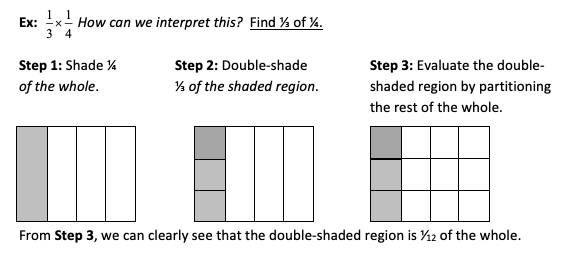
\includegraphics[width=1\linewidth]{images/frac-mult-rect.png}
\end{sbspanel}%
\end{sidebyside}%
\par
NOTE \#1: Your final answer might not be in its most simplified form after Step 3. So simplify it! NOTE \#2: You can perform all three steps within one whole.%
\end{introduction}%
\begin{divisionexercise}{1}{}{}{g:exercise:idm35280853360}%
\(\frac{2}{5} \times \frac{1}{3} \)%
\begin{sidebyside}{1}{0.2}{0.2}{0}%
\begin{sbspanel}{0.6}%
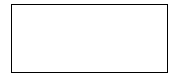
\includegraphics[width=1\linewidth]{images/generic-rectangle.png}
\end{sbspanel}%
\end{sidebyside}%
\end{divisionexercise}%
\clearpage
\begin{divisionexercise}{2}{}{}{g:exercise:idm35278777168}%
\(\frac{3}{4} \times \frac{5}{6} \)%
\begin{sidebyside}{1}{0.2}{0.2}{0}%
\begin{sbspanel}{0.6}%
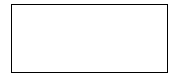
\includegraphics[width=1\linewidth]{images/generic-rectangle.png}
\end{sbspanel}%
\end{sidebyside}%
\end{divisionexercise}%
\clearpage
\begin{introduction}{}%
Exploration 2: Fraction Multiplication with Pattern Blocks. (NOTE: For the entire exploration, two hexagons is the whole.)%
\begin{sidebyside}{1}{0}{0}{0}%
\begin{sbspanel}{1}%
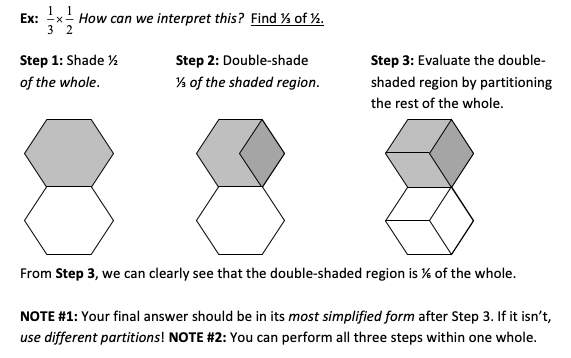
\includegraphics[width=1\linewidth]{images/frac-mult-pattern.png}
\end{sbspanel}%
\end{sidebyside}%
\par
NOTE \#1: Your final answer might not be in its most simplified form after Step 3. So simplify it! NOTE \#2: You can perform all three steps within one whole.%
\end{introduction}%
\begin{divisionexercise}{3}{}{}{g:exercise:idm35279179952}%
\(\frac{2}{3} \times \frac{1}{4} \)%
\begin{sidebyside}{1}{0.1}{0.1}{0}%
\begin{sbspanel}{0.8}%
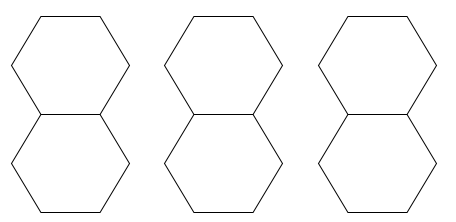
\includegraphics[width=1\linewidth]{images/3-double-hexagons.png}
\end{sbspanel}%
\end{sidebyside}%
\end{divisionexercise}%
\clearpage
\begin{divisionexercise}{4}{}{}{g:exercise:idm35280017552}%
\(\frac{1}{3} \times \frac{3}{4} \)%
\begin{sidebyside}{1}{0.1}{0.1}{0}%
\begin{sbspanel}{0.8}%
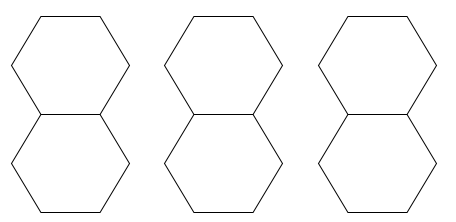
\includegraphics[width=1\linewidth]{images/3-double-hexagons.png}
\end{sbspanel}%
\end{sidebyside}%
\end{divisionexercise}%
\begin{divisionexercise}{5}{}{}{g:exercise:idm35280401856}%
\(\frac{5}{6} \times \frac{1}{2} \)%
\begin{sidebyside}{1}{0.1}{0.1}{0}%
\begin{sbspanel}{0.8}%
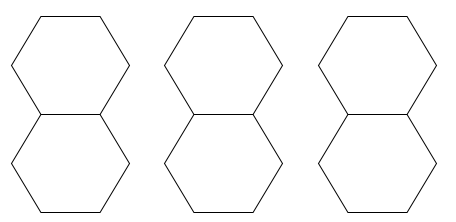
\includegraphics[width=1\linewidth]{images/3-double-hexagons.png}
\end{sbspanel}%
\end{sidebyside}%
\end{divisionexercise}%
\begin{divisionexercise}{6}{}{}{g:exercise:idm35280323792}%
\(\frac{1}{3} \times \frac{1}{4} \)%
\begin{sidebyside}{1}{0.1}{0.1}{0}%
\begin{sbspanel}{0.8}%
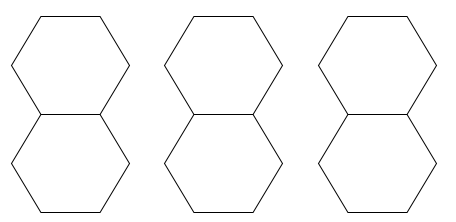
\includegraphics[width=1\linewidth]{images/3-double-hexagons.png}
\end{sbspanel}%
\end{sidebyside}%
\end{divisionexercise}%
\end{worksheet-section-numberless}
\restoregeometry
%
%
\typeout{************************************************}
\typeout{Worksheet 0 Multiplying Decimals}
\typeout{************************************************}
%
\newgeometry{left=1.25cm, right=1.25cm, top=1.25cm, bottom=1.25cm}
\begin{worksheet-section-numberless}{Multiplying Decimals}{}{Multiplying Decimals}{}{}{x:worksheet:ws-mult-decimals}
\begin{divisionexercise}{1}{}{}{g:exercise:idm35304290992}%
Using decimal squares show 3 groups of 0.12 (i.e., 3×0.12).%
\begin{sidebyside}{1}{0.25}{0.25}{0}%
\begin{sbspanel}{0.5}%

\includegraphics[width=1\linewidth]{images/decimal-square.png}
\end{sbspanel}%
\end{sidebyside}%
\end{divisionexercise}%
\begin{divisionexercise}{2}{}{}{g:exercise:idm35304310960}%
Model the following multiplication expressions using decimal squares and find the answers. In each case explain how regrouping shows up both in the arithmetic operation and in the picture.%
%
\begin{enumerate}[label=(\alph*)]
\item{}\(4 \times 0.9 \)%
\item{}\(3 \times 0.74 \)%
\end{enumerate}
\end{divisionexercise}%
\begin{divisionexercise}{3}{}{0.1}{g:exercise:idm35304340880}%
Explain how using decimal squares helps explain where to put the decimal point in the following problems:%
%
\begin{enumerate}[label=(\alph*)]
\item{}\(10 \times 0.2 \)%
\item{}\(10 \times 0.12 \)%
\item{}\(100 \times 0.03 \)%
\end{enumerate}
\end{divisionexercise}%
\begin{divisionexercise}{4}{}{}{g:exercise:idm35304379728}%
Model the following multiplication expressions using decimal squares and find the answers. (Recall the definition of multiplication)%
%
\begin{enumerate}[label=(\alph*)]
\item{}\(\frac{1}{2} \times 0.8 \)%
\item{}\(\frac{3}{4} \times 0.16 \)%
\end{enumerate}
\end{divisionexercise}%
\clearpage
\begin{introduction}{}%
Model the following multiplication expressions using an area model and find the answers.  Make sure that you can explain how you know where the decimal place goes.%
\end{introduction}%
\begin{divisionexercise}{5}{}{}{g:exercise:idm35277977184}%
\(0.4 \times 0.16\)%
\end{divisionexercise}%
\begin{divisionexercise}{6}{}{}{g:exercise:idm35277999920}%
\(1.2 \times 0.8\)%
\end{divisionexercise}%
\begin{divisionexercise}{7}{}{}{g:exercise:idm35278021488}%
\(2.3 \times 3.7 \)%
\end{divisionexercise}%
\end{worksheet-section-numberless}
\restoregeometry
%
%
\typeout{************************************************}
\typeout{Worksheet 0 Meaning of Division}
\typeout{************************************************}
%
\newgeometry{left=1.25cm, right=1.25cm, top=1.25cm, bottom=1.25cm}
\begin{worksheet-section-numberless}{Meaning of Division}{}{Meaning of Division}{}{}{x:worksheet:ws-div-meaning}
\begin{introduction}{}%
\begin{sidebyside}{1}{0}{0}{0}%
\begin{sbspanel}{1}%
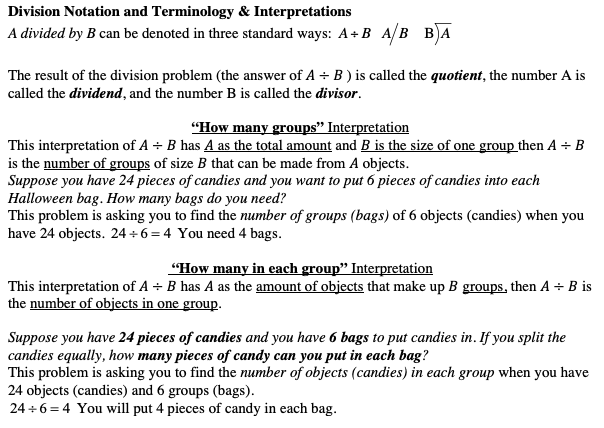
\includegraphics[width=1\linewidth]{images/div-meaning.png}
\end{sbspanel}%
\end{sidebyside}%
%
\par
Exploration 1: For the following story problems, write the corresponding numerical division expression (e.g.,  24÷6 ), decide what each number represents and which interpretation of division is involved. Find the quotient!%
\end{introduction}%
\begin{divisionexercise}{1}{}{0.04}{g:exercise:idm35303528176}%
The month of February in 2018 has 28 days. How many weeks are there in February 2018?%
\end{divisionexercise}%
\begin{divisionexercise}{2}{}{0.04}{g:exercise:idm35303595568}%
If you drive 324 miles at a constant speed for 6 hours, then how fast did you go?%
\end{divisionexercise}%
\begin{divisionexercise}{3}{}{0.04}{g:exercise:idm35303651856}%
The month of February in 2018 has 28 days. How many weeks are there in February 2018?%
\end{divisionexercise}%
\begin{divisionexercise}{4}{}{}{g:exercise:idm35303686528}%
If 75 fluid ounces of mouthwash costs \textdollar{}5, then how much of this mouthwash will you get for \textdollar{}1?%
\end{divisionexercise}%
\clearpage
\begin{introduction}{}%
Exploration 2: Write an expression involving division that would correspond to the following problems and find the answer if possible.%
\end{introduction}%
\begin{divisionexercise}{5}{}{0.1}{g:exercise:idm35278027328}%
I have 0 candies.  I want to make goodie bags with 5 candies each.  How many goodie bags can I make?%
\end{divisionexercise}%
\begin{divisionexercise}{6}{}{0.1}{g:exercise:idm35304384784}%
I have 20 candies.  I want to make goodie bags with 0 candies each.  How many goodie bags can I make?%
\end{divisionexercise}%
\begin{introduction}{}%
Exploration 3: Solve each of the following problems. Explain how the context affects what form the answer might take.%
\end{introduction}%
\begin{divisionexercise}{7}{}{0.1}{g:exercise:idm35277982960}%
Nicole has 100 Halloween stickers that need to be distributed to her 32 students. How many stickers does each student receive?%
\end{divisionexercise}%
\begin{divisionexercise}{8}{}{0.1}{g:exercise:idm35304346704}%
Marci has 100 second graders who are going to the zoo. Each bus will hold 32 students. How many buses does she need?%
\end{divisionexercise}%
\begin{divisionexercise}{9}{}{0.1}{g:exercise:idm35304326000}%
Olivia has 100 square yards to make ghost costumes for Halloween. She needs to make 32 ghost costumes. How much material does she have for each costume?%
\end{divisionexercise}%
\end{worksheet-section-numberless}
\restoregeometry
%
%
\typeout{************************************************}
\typeout{Worksheet 0 Dividing Fractions}
\typeout{************************************************}
%
\newgeometry{left=1.25cm, right=1.25cm, top=1.25cm, bottom=1.25cm}
\begin{worksheet-section-numberless}{Dividing Fractions}{}{Dividing Fractions}{}{}{x:worksheet:ws-div-frac-1}
\begin{introduction}{}%
Exploration 1: Discuss how many \(\frac{1}{2} \) (halves) there are in one whole. How many are in 2 wholes, or 3 wholes? Draw pictures to illustrate your thinking and your answers. How do you know you are correct? Represent your answers using equations.%
\end{introduction}%
\end{worksheet-section-numberless}
\restoregeometry
%
%
\typeout{************************************************}
\typeout{Worksheet 0 Dividing Fractions Part 2}
\typeout{************************************************}
%
\newgeometry{left=1.25cm, right=1.25cm, top=1.25cm, bottom=1.25cm}
\begin{worksheet-section-numberless}{Dividing Fractions Part 2}{}{Dividing Fractions Part 2}{}{}{x:worksheet:ws-div-frac-2}
\begin{introduction}{}%
Exploration 2: Use one of the models (Cuisenaire rods, fraction bars, fraction models, rectangles, pattern blocks, double number lines, etc.) to answer the following questions. Discuss which interpretation of division is suitable for each problem.%
\end{introduction}%
\begin{divisionexercise}{1}{}{0.2}{g:exercise:idm35280608528}%
A carton containing \(\frac{1}{2} \)  a quart of cream is used to fill creamers that hold \(\frac{1}{6} \)  quart each.  How many creamers can be filled?%
\end{divisionexercise}%
\begin{divisionexercise}{2}{}{0.2}{g:exercise:idm35303246832}%
A cookie recipe calls for \(\frac{1}{3} \) cup of sugar for one batch.  If you have \(\frac{1}{2} \) a cup of sugar, how many batches of cookies can you make?%
\end{divisionexercise}%
\begin{divisionexercise}{3}{}{0.2}{g:exercise:idm35280592672}%
Katie wants to make a recipe that calls for \(2 \frac{1}{2} \) cups of flour but finds that she only has \(1 \frac{3}{4} \) cups of flour. Assuming she wants to keep all the ingredient ratios the same as in the recipe, what fraction of the recipe can she make?%
\end{divisionexercise}%
\clearpage
\begin{divisionexercise}{4}{}{0.2}{g:exercise:idm35279334768}%
You used 6 cans of paint for 3 walls, how many cans of paint do you need to paint one wall?  What if you used \(\frac{3}{4} \) of a can to paint \(\frac{2}{3} \) of a wall. How many cans of paint do you need to paint one wall?%
\end{divisionexercise}%
\begin{divisionexercise}{5}{}{0.2}{g:exercise:idm35279728320}%
If \(\frac{1}{4} \)  cup of water fills \(\frac{1}{3} \)  of a plastic container, then how much water will the full container hold?%
\end{divisionexercise}%
\begin{divisionexercise}{6}{}{0.2}{g:exercise:idm35257887744}%
If you have \(\frac{3}{4} \) pound of candy and you divide the candy in half, how much candy will you have in each portion? What if, you have \(\frac{3}{4} \) pound of candy and you divide the candy by half, how much candy will you have in each?%
\end{divisionexercise}%
\clearpage
\begin{divisionexercise}{7}{}{0.2}{g:exercise:idm35257884672}%
Explain why when is 4 divided by 8, the quotient is less than 4, but when \(\frac{1}{4} \)  is divided by \(\frac{1}{8} \) , the quotient is greater than \(\frac{1}{4} \)?%
\end{divisionexercise}%
\end{worksheet-section-numberless}
\restoregeometry
%
%
\typeout{************************************************}
\typeout{Worksheet 0 Dividing Fractions Part 3}
\typeout{************************************************}
%
\newgeometry{left=1.25cm, right=1.25cm, top=1.25cm, bottom=1.25cm}
\begin{worksheet-section-numberless}{Dividing Fractions Part 3}{}{Dividing Fractions Part 3}{}{}{x:worksheet:ws-div-frac-3}
\begin{introduction}{}%
Dividing Fractions with Pattern Blocks. (Use TWO yellow hexagons as the whole for the entire exploration.)%
\begin{sidebyside}{1}{0}{0}{0}%
\begin{sbspanel}{1}%
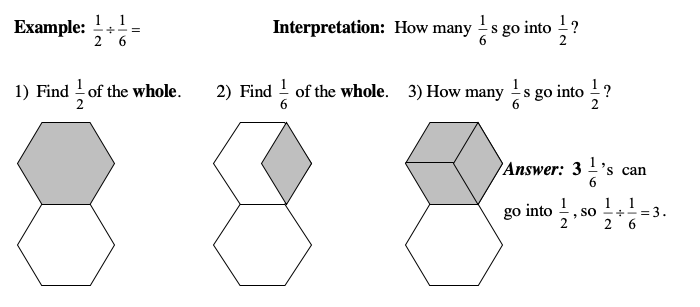
\includegraphics[width=1\linewidth]{images/frac-div-hex-1.png}
\end{sbspanel}%
\end{sidebyside}%
\end{introduction}%
\begin{divisionexercise}{1}{}{}{g:exercise:idm35257843168}%
\(\frac{3}{4} \div \frac{1}{12} \)%
\begin{sidebyside}{1}{0.15}{0.15}{0}%
\begin{sbspanel}{0.7}%
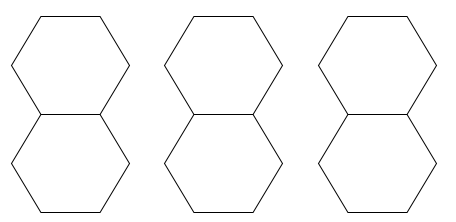
\includegraphics[width=1\linewidth]{images/3-double-hexagons.png}
\end{sbspanel}%
\end{sidebyside}%
\end{divisionexercise}%
\clearpage
\begin{introduction}{}%
\begin{sidebyside}{1}{0}{0}{0}%
\begin{sbspanel}{1}%
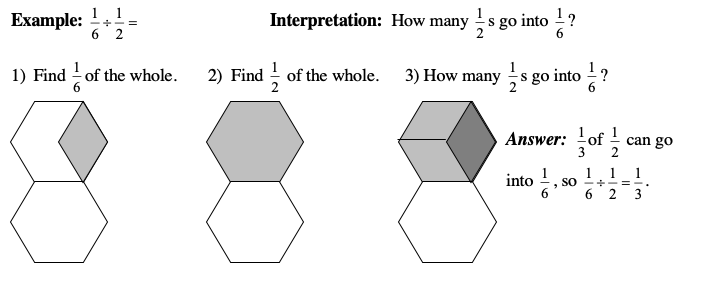
\includegraphics[width=1\linewidth]{images/frac-div-hex-2.png}
\end{sbspanel}%
\end{sidebyside}%
\end{introduction}%
\begin{divisionexercise}{2}{}{}{g:exercise:idm35257838432}%
\(\frac{1}{2} \div \frac{3}{4} \)%
\begin{sidebyside}{1}{0.15}{0.15}{0}%
\begin{sbspanel}{0.7}%
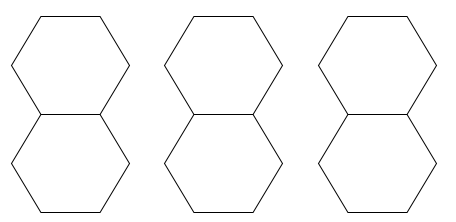
\includegraphics[width=1\linewidth]{images/3-double-hexagons.png}
\end{sbspanel}%
\end{sidebyside}%
\end{divisionexercise}%
\clearpage
\begin{introduction}{}%
\begin{sidebyside}{1}{0}{0}{0}%
\begin{sbspanel}{1}%
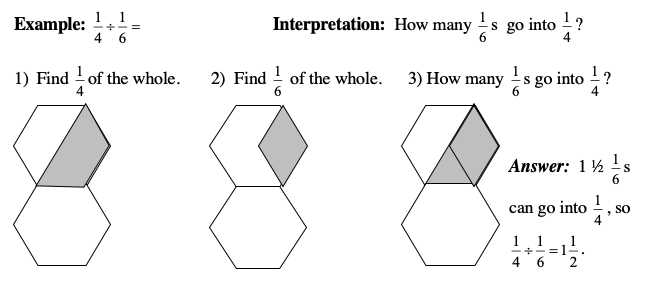
\includegraphics[width=1\linewidth]{images/frac-div-hex-3.png}
\end{sbspanel}%
\end{sidebyside}%
\end{introduction}%
\begin{divisionexercise}{3}{}{}{g:exercise:idm35257833696}%
\(\frac{3}{4} \div \frac{5}{12} \)%
\begin{sidebyside}{1}{0.15}{0.15}{0}%
\begin{sbspanel}{0.7}%
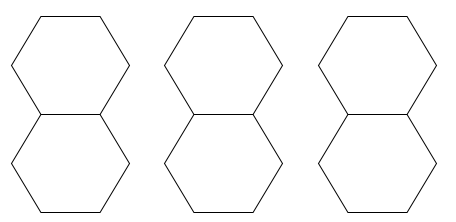
\includegraphics[width=1\linewidth]{images/3-double-hexagons.png}
\end{sbspanel}%
\end{sidebyside}%
\end{divisionexercise}%
\end{worksheet-section-numberless}
\restoregeometry
%
%
\typeout{************************************************}
\typeout{Worksheet 0 Dividing Fractions Part 4}
\typeout{************************************************}
%
\newgeometry{left=1.25cm, right=1.25cm, top=1.25cm, bottom=1.25cm}
\begin{worksheet-section-numberless}{Dividing Fractions Part 4}{}{Dividing Fractions Part 4}{}{}{x:worksheet:ws-div-frac-4}
\begin{introduction}{}%
Exploration 4: Dividing Fractions with Rectangles.  Refer to the examples provided in class and Exploration \#1 to illustrate the following problems.  In each problem, one rectangle is the whole.%
\end{introduction}%
\begin{divisionexercise}{1}{}{0.1}{g:exercise:idm35257873168}%
\(\frac{2}{3} \div \frac{1}{6} \)%
\begin{sidebyside}{1}{0.1}{0.1}{0}%
\begin{sbspanel}{0.8}%
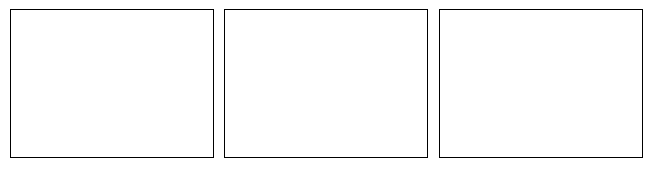
\includegraphics[width=1\linewidth]{images/3-rectangles.png}
\end{sbspanel}%
\end{sidebyside}%
\end{divisionexercise}%
\begin{divisionexercise}{2}{}{0.1}{g:exercise:idm35257829264}%
\(\frac{5}{6} \div \frac{2}{5} \)%
\begin{sidebyside}{1}{0.1}{0.1}{0}%
\begin{sbspanel}{0.8}%
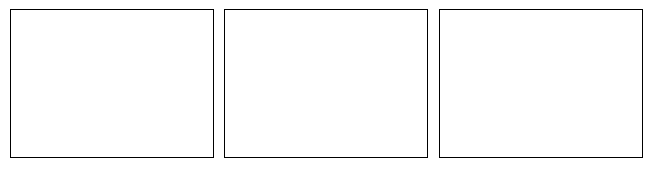
\includegraphics[width=1\linewidth]{images/3-rectangles.png}
\end{sbspanel}%
\end{sidebyside}%
\end{divisionexercise}%
\begin{divisionexercise}{3}{}{0.1}{g:exercise:idm35257826160}%
\(\frac{2}{5} \div \frac{3}{4} \)%
\begin{sidebyside}{1}{0.1}{0.1}{0}%
\begin{sbspanel}{0.8}%
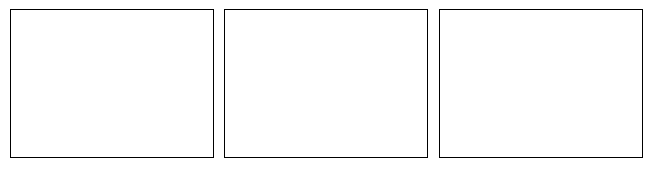
\includegraphics[width=1\linewidth]{images/3-rectangles.png}
\end{sbspanel}%
\end{sidebyside}%
\end{divisionexercise}%
\end{worksheet-section-numberless}
\restoregeometry
\end{chapterptx}
\end{document}